\documentclass[12pt]{article}
\usepackage[utf8]{inputenc}
\usepackage{graphicx}
\usepackage{braket}
\usepackage{amsmath}
\usepackage{feynmf}
\usepackage{listings}
\newcommand{\HRule}{\rule{\linewidth}{0.5mm}}
\addtolength{\oddsidemargin}{-1in}
\addtolength{\evensidemargin}{-1in}
\addtolength{\textwidth}{2in}

\addtolength{\topmargin}{-.875in}
\addtolength{\textheight}{1.75in}

\pagenumbering{gobble}

\renewcommand{\thefootnote}{\fnsymbol{footnote}}
\title{A simulation study of neutrino oscillations in the Long Baseline Neutrino Experiment}
\author{Sam Bloom }
\date{April 2015}

\begin{document}
\begin{titlepage}
\begin{center}

% Upper part of the page. The '~' is needed because \\
% only works if a paragraph has started.
\includegraphics[width=0.15\textwidth]{./logo}~\\[1cm]

\textsc{\LARGE University of Sussex}\\[1.5cm]
\begin{center}
\includegraphics[scale=0.4]{University_of_Sussex_Coat_of_Arms.pdf}
\begin{figure}[h!]
\end{figure}
\end{center}
\textsc{\Large Final year project}\\[0.5cm]

% Title
\HRule \\[0.1cm]
\vspace{-4mm}
\HRule \\[0.4cm]
{ \huge \bfseries A simulation study of neutrino oscillations in the Long Baseline Neutrino Experiment \\[0.4cm] }

\HRule \\[0.1cm]
\vspace{-4mm}
\HRule \\[1.5cm]

% Author and supervisor
\noindent
\begin{minipage}[t]{0.4\textwidth}
\begin{flushleft} \large
\emph{Candidate number:}\\
\textsc{75580}
\end{flushleft}
\end{minipage}%
\begin{minipage}[t]{0.4\textwidth}
\begin{flushright} \large
\emph{Supervisor:} \\
Dr.~Elisabeth \textsc{Falk}
\end{flushright}
\vspace{10mm}
\end{minipage}

\begin{abstract}
\begin{center}
\noindent The phenomenology of neutrino oscillations is explored, including the effect of the neutrino mass hierarchy, matter effect, and a possible non-zero CP violating phase. The principles of existing neutrino experiments are outlined and the sensitivity of the Long Baseline Neutrino Experiment to the true mass hierarchy and CP violation is modelled.
\end{center}
\end{abstract}

\vfill
% Bottom of the page
{\large May 7, 2015}
\end{center}
\end{titlepage}
\section*{Preface}
This project explores the phenomenology of neutrino oscillations in the context of the Long Baseline Neutrino Experiment (LBNE). Expressions for oscillation and appearance probabilities are derived and are used to generate figures, simulated signals and sensitivity predictions. The effect of the known mixing parameters, the mass hierarchy, the CP violating phase and matter, are all detailed and taken into account. All figures were generated using code written by myself in Python, unless otherwise stated. An example of the Python code used to obtain results is displayed in the Appendix. Diagrams were produced by myself. The design and principles of the LBNE are outlined, and I model the predicted sensitivity of the experiment to the true neutrino mass hierarchy and CP violating phase.
\newpage
\tableofcontents
\pagenumbering{arabic}
\newpage
\section{Neutrinos}
\subsection{Discovery}
The existence of the neutrino was first indicated in 1914 by the observation of the beta decay energy spectrum. In beta decay, a nucleus emits an electron or a positron, referred to as beta particles. James Chadwick showed that the energy of the beta particle appears to take a continuous range of values, as opposed to having a discrete energy\cite{Close}. At the time this was unexpected, because if the beta particle was the only particle emitted, it should only be able to take on one particular energy, due to conservation of energy and momentum.\\\\
In Wolfgang Pauli's famous 1930 letter\cite{Close}, he attempted to explain the anomalous beta spectrum as well as another contemporary nuclear physics problem known as the `nitrogen anomaly'. His solution was the existence of a light neutral particle, which he called the neutron. Controversially, it had to be nearly impossible to detect, to explain why it had yet to be seen. The neutron as we know it today had not yet been discovered at the time of Pauli's letter, so it seemed plausible that the proposal would explain the two mysteries at once. However in 1932, James Chadwick discovered a neutral particle in the atomic nucleus, and showed that it had a similar mass to the proton\cite{Close}. This indicated that the neutron that Pauli proposed to answer the nitrogen anomaly could not be the same one that explained the anomalous beta spectrum.\\\\
Enrico Fermi later formed a theory of beta decay using Pauli's proposed particle. He coined the term `neutrino', meaning `little neutron', to distinguish it from the neutron\cite{Close}. It wasn't until 1956 that the neutrino was proven to exist by direct detection. Clyde L. Cowan and Frederick Reines performed an experiment using inverse beta decay- the process in which a proton absorbs an electron antineutrino, producing a neutron and a positron. Through this process they were able to successfully detect electron antineutrinos produced by a nuclear reactor\cite{Cowan}.\\\\
In 1962 the muon neutrino was discovered by Lederman, Schwartz and Steinberger\cite{Lederman}, who used a synchotron to produce pions. These pions would decay to muons, and these muons would be stopped by a thick steel wall. A spark chamber on the other side of this steel wall detected muons, even though none could penetrate the wall. This proved that muon neutrinos were being produced, which were producing muons when they interacted in the spark chamber.\\\\
The tau neutrino was discovered in 1997 by the Direct Observation of Nu Tau (DONuT) experiment at Fermilab, Illinois\cite{tau}. The tau neutrinos were produced by the decay of charmed mesons from the Tevatron proton accelerator. The experiment searched for particle tracks characteristic of a tau lepton, which would appear out of nowhere and suddenly deviate after a very short distance as the tau decayed.
\subsection{Properties}
An electron neutrino owes its name to the fact that it is associated with an electron flavoured charged lepton, i.e. an electron or positron is observed in its interactions. So the antineutrinos detected by Cowan and Reines were 'electron flavoured'. In the following years the muon and tau neutrinos, as well as their antineutrino counterparts, were discovered. The Standard Model of particle physics currently includes six types of neutrino; three flavours and their antiparticles.\\\\
Neutrinos are very difficult to detect due to the fact that they only interact through the weak interaction. They interact so rarely that, on Earth, roughly sixty-five billion solar neutrinos pass through a square centimeter every second\cite{PDG}, yet their presence is completely unnoticed. This makes studying neutrinos very challenging, as they cannot simply be tracked or contained- they tend to just pass straight through detectors, with a few very rare interaction events. Therefore typical neutrino experiments require enormous detector volumes or very high neutrino fluxes, often both, in order to produce a statistically significant amount of data.\\\\
The Standard Model has for a long time assumed the mass of the neutrino to be zero. Current attempts at directly measuring the neutrino mass have all failed to set a lower limit distinguishable from zero, so until recently it was generally accepted that the neutrino was massless. However the phenomenon known as neutrino oscillation has proven that neutrinos do in fact have non-zero mass, and that there are three distinct neutrino masses.\\\\
\subsection{The solar neutrino problem}
The Sun produces neutrinos in nuclear fusion reactions, which there have been many attempts to model. There are many different types of fusion reaction taking place in the Sun, producing neutrinos with signature energies. The relative fluxes of these neutrinos indicate the rates at which these processes occur. In the late 1960s Raymond Davis Jr and John N. Bahcall lead an experiment at Homestake Mine in South Dakota, in which they attempted to measure the total flux of neutrinos from nuclear fusion in the Sun. The standard solar model gave a good prediction of how many neutrinos to expect on Earth, and Bahcall had calculated the total rate that they could expect to measure from their detector. The rate observed came to be about a third of that expected with no indication of a systematic error in the experiment, so this pointed to some new physics\cite{Martin}. The problem became known as the solar neutrino problem.\\\\
Bruno Pontecorvo proposed a solution to this problem in 1968 by suggesting that neutrinos might in fact have mass, allowing a neutrino of one type to change to a neutrino of another type, between the time it is produced and the time it reaches Earth\cite{Pontecorvo}. In other words, neutrinos oscillate. An electron neutrino produced in the Sun would therefore be allowed to change into another type, for example a muon neutrino, which the detector is not sensitive to. If some of the solar neutrinos were changing to other types, and therefore not being detected, this could account for the discrepancy measured by Davis and Bahcall.\\\\
Evidence of neutrino oscillation came a very long time after Pontecorvo's proposal, in the form of solar neutrinos at Sudbury Neutrino Observatory (SNO) in 2001. SNO detected all three flavours of neutrino coming from the Sun, and was able to distinguish whether they were electron neutrinos, or either muon or tau neutrinos, which the Sun cannot produce. The results confirmed Bahcall's calculations as well as Pontecorvo's proposal and showed that the missing electron neutrinos had taken the form of muon and tau neutrinos by neutrino oscillation\cite{SNO1}.
\section{Neutrino oscillations}
There are three types of neutrino that can be detected, called electron, muon and tau neutrinos, but this does not convey their true nature. What is meant by the term `electron neutrino' is a neutrino whose interactions are `electron-like', i.e. there is also an electron or positron present in that interaction. So a neutrino whose interactions produce muons would be described as `muon-like', and would therefore be called a muon neutrino. When neutrinos were less well understood this seemed like an appropriate way of labelling the three types, because it was thought that lepton flavour was a conserved quantity. However the discovery of neutrino oscillations showed that this is not the case, and that a neutrino cannot be defined by its flavour alone.\\\\
In reality, flavour is only one way of looking at a neutrino, the other is mass. There are three distinct mass states a neutrino can have, and one might assume that these mass states correspond to the three flavour states, much like in the case of charged leptons, where the electron is the lightest mass state and the tau is the heaviest. However the key to understanding the way neutrinos oscillate is the fact that their mass states do not correspond to the flavour states- each flavour state is a superposition of all three mass states. Each flavour of neutrino is a flavour eigenstate- a basis state of the weak interaction, but each neutrino mass state is an eigenstate of mass. When a neutrino is produced in a weak interaction, it is in a definite flavour eigenstate, i.e. if it were to be instantly observed in another weak interaction, there is a one hundred percent probability of observing that flavour. However its mass state is undetermined because it is in a superposition of all three mass eigenstates. Each mass eigenstate propagates with a different phase, so when a neutrino produced in a definite flavour eigenstate propagates, the mixture of mass states evolves in time, causing its flavour state to no longer be determined. So an electron neutrino produced by a nuclear fusion reaction in the Sun could be detected as a muon neutrino, with a probability depending on how long it has been propagating, and therefore the distance it has travelled. This is why SNO detected muon and tau neutrinos coming from the Sun- they all started their journey as electron neutrinos, but on their way to Earth their mass states propagated with different phases, so their probability of being detected as electron neutrinos decreased, in favour of the other flavours. Figure \ref{fig:mixing} illustrates how each mass state is a different mixture of flavour states.
\begin{center}
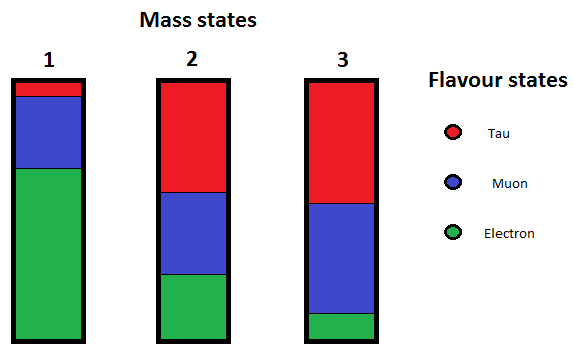
\includegraphics[scale=0.5]{mixing.png}
\begin{figure}[h!]
\caption{The three neutrino mass states showing their unique flavour compositions.}
\label{fig:mixing}
\end{figure}
\end{center}
\subsection{Derivation of two flavour oscillation probability}
The following derivation is described in detail in \cite{Giunti} and has been adapted by myself. The state of a neutrino after being produced in a weak interaction process is a pure flavour state $\alpha$ described by a weighted sum of each mass state $k$.\begin{gather}
$$\ket{\nu_\alpha}=\sum\limits_{k}U_{\alpha k}^*\ket{\nu_k}$$.\label{eq:1}
\end{gather}
The weightings here are elements of a mixing matrix $U$, such as the one mentioned in equation \ref{eq:U}. Each mass state  evolves with time $t$ and energy $E_k$ such that\begin{gather}
$$\ket{{\nu_{k}(t)}}=e^{-iE_{k}t}\ket{{\nu_{k}}}$$.
\label{eq:2}
\end{gather}
Equation \ref{eq:1} can be inverted to show how mass states can be seen as superpositions of flavour eigenstates\begin{gather}
$$ \ket{\nu_k}=\sum\limits_{\alpha}U_{\alpha k}\ket{\nu_\alpha}  $$.
\label{eq:3}
\end{gather}
Equations \ref{eq:1} and \ref{eq:2} can be combined to show how a flavour state evolves with time, in terms of mass eigenstates\begin{gather}
$$\ket{{\nu_{\alpha}(t)}}=\sum\limits_{k}U_{\alpha k}^*e^{-iE_{k}t}\ket{{\nu_{k}}}$$.
\label{eq:4}
\end{gather}\\
Now equation \ref{eq:3} can be substituted into equation \ref{eq:4} to show how the flavour state of a neutrino at time $t$ is related to a particular flavour eigenstate\begin{gather}
$$\ket{{\nu_{\alpha}(t)}}=\sum\limits_{\beta}(\sum\limits_{k}U_{\alpha k}^*e^{-iE_{k}t}U_{\beta k})\ket{\nu_{\beta}}$$.
\label{eq:5}
\end{gather}\\
The amplitude of the transition $\nu_\alpha \rightarrow \nu_\beta$ is given by
\begin{gather}
$$A_{\nu_\alpha \rightarrow \nu_\beta}(t)=\braket{\nu_\beta|\nu_{\alpha}(t)}=\sum\limits_{k}U_{\alpha k}^*U_{\beta k}e^{-iE_{k}t}$$.
\label{eq:6}
\end{gather}\\
The probability of the transition $\nu_\alpha \rightarrow \nu_\beta$ is the square of the modulus of the amplitude therefore\begin{gather}
$$P{_\nu_\alpha \rightarrow \nu_\beta}(t)=\braket{\nu_\beta|\nu_{\alpha}(t)}=\sum\limits_{k,j}U_{\alpha k}^*U_{\beta k}U_{\alpha j}U_{\beta j}^*e^{-i(E_{k}-E_{j})t}$$.
\label{eq:7}
\end{gather}\\
A particle of mass $m_{k}$ and momentum $\vec{p}$ has energy\begin{gather}
$$ E_{k}=\sqrt{m_{k}^2+\vec{p}^2} $$.
\label{eq:8}
\end{gather}\\
However, neutrinos are typically relativistic, and their masses are so small that $\frac{m_{k}^2}{\vec{p}^2} << 1$ and $E\simeq|\vec{p}|$. Therefore, the energy of a neutrino can be approximated as\begin{gather}
$$ E_{k}\simeq E+\frac{m_{k}^2}{2E} $$.
\label{eq:9}
\end{gather}
The difference between two relativistic neutrino energies is therefore approximated by\begin{gather}
$$ E_{k}-E_{j}\simeq \frac{\Delta m_{kj}^2}{2E}, & &\Delta m_{kj}^2=\Delta m_{k}^2-\Delta m_{j}^2 $$.
\label{eq:10}
\end{gather}\\
Working in natural units $t=L$, so it is possible to express the total probability of the transition $\nu_\alpha \rightarrow \nu_\beta$ in a vacuum, as a function of $L$ and $E$
\begin{gather}
P_{\nu_{\alpha} \rightarrow \nu_\beta}(L,E)=\braket{\nu_\beta|\nu_{\alpha}(t)}=\sum\limits_{k,j}U_{\alpha k}^*U_{\beta k}U_{\alpha j}U_{\beta j}^*e^{\frac{-i\Delta m_{kj}^2L}{2E}}.
\label{eq:11}
\end{gather}
For the case of two neutrino flavours and two neutrino masses, the mixing matrix is
\begin{align}U=\begin{bmatrix}
\cos{\theta}&\sin{\theta}\\-\sin{\theta}&\cos{\theta}
\end{bmatrix}.
\label{eq:U}
\end{align}
In a two neutrino scenario, where the flavours being considered are $\mu$ and $e$, the mixing angle of interest is $\theta_{12}$ and the mass splitting is given by $\Delta m_{21}^2\equiv m_{2}^2-m_{1}^2$. By substituting in the matrix elements from equation $12$ into equation $11$ and with some rearrangement the two flavour oscillation probability for a muon neutrino is
\begin{gather}
P_{\nu_{\mu} \rightarrow \nu_e}(L,E)=\sin^{2}(2\theta_{12})\sin^{2}(\frac{\Delta m_{21}^2L}{4E}).
\label{eq:2flavour}
\end{gather}
This formula shows the effects of the mixing angle $\theta_{12}$ and the mass splitting $\Delta m_{12}^2$. The mixing angle determines the amplitude of the oscillation and the mass splitting determines the period. The probability of detecting an electron neutrino oscillates with $L/E$. The survival probability is simply given by $P_{\nu_{\mu} \rightarrow \nu_\mu}=1-P_{\nu_{\mu} \rightarrow \nu_e}$. Figure \ref{fig:oscillationandsurvival} illustrates how both probabilities look over a range of values of $L/E$.
\begin{figure}[h!]
    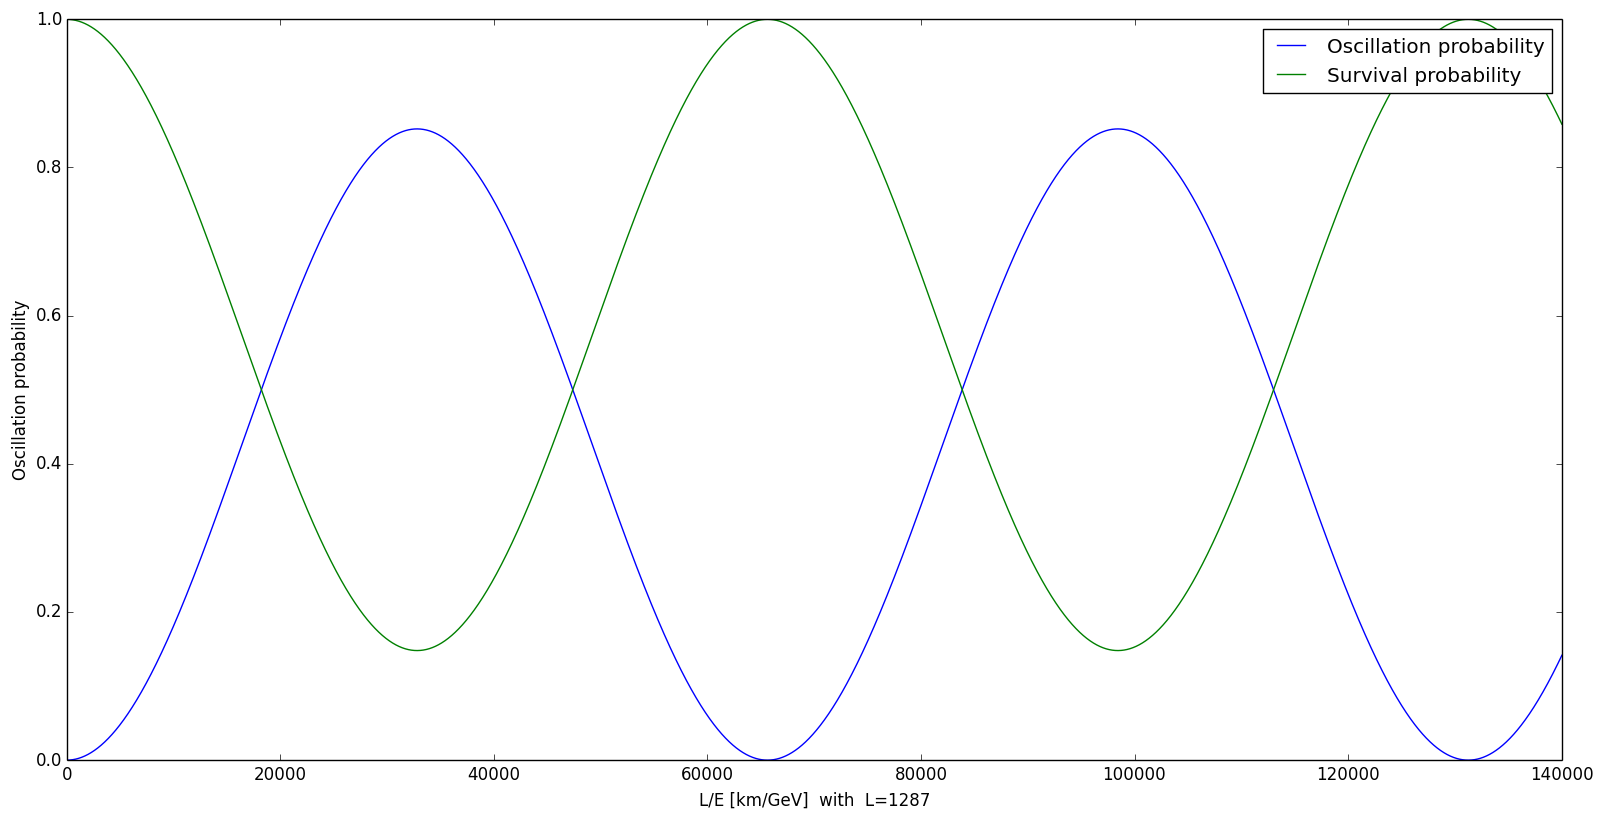
\includegraphics[scale=0.4]{2_flavour_no_matter.png}
\caption{Oscillation and survival probabilities for muon and electron neutrinos as a function of energy and distance, in the case of two flavour mixing.}
\label{fig:oscillationandsurvival}
\end{figure}\\\\
\newpage
\subsection{Mixing parameters}
At present the standard model includes three active neutrinos, so the two flavour oscillation probabilities are only approximate. To know the true probability of detecting a particular neutrino, one must consider all three neutrino flavours. This introduces more parameters- three mixing angles, three mass splittings and a CP violating phase.\\\\
\subsubsection{Mass differences}
In a three neutrino model, there are three independent neutrino masses. The absolute values of these masses are not known, due to their very small magnitudes. However neutrino oscillation experiments are able to determine the differences in these masses. Conventionally, the mass differences are defined by\cite{PDG}:
\begin{align}
\Delta m_{kj}^2\equiv m_{k}^2-m_{j}^2,\\
\Delta M^2\equiv m_3^2-\frac{m_2^2+m_1^2}{2}.
\end{align}
It then follows that the remaining mass differences are given by
\begin{align}
\Delta m_{31}^2= \Delta M^2 +\frac{\Delta m_{21}^2}{2},\\
\Delta m_{32}^2= \Delta M^2 -\frac{\Delta m_{21}^2}{2}.
\end{align}
$m_2$ is by definition larger than $m_1$, and these two masses are very close together compared to $m_3$. It is not known whether $m_3$ is larger than $m_1$ or $m_2$. The quantity $\Delta M^2$ represents the average difference between $m_3$ and $m_1$ and $m_2$. $\Delta m_{21}^2$ and the magnitude of $\Delta M^2$ have been measured, but the sign of $\Delta M^2$ is unknown. The ambiguity in the sign of $\Delta M^2$ is referred to as the neutrino mass hierarchy, and is illustrated in figure \ref{fig:hierarchy_demo}. If $m_1<m_2<m_3$ then the hierarchy is said to be normal, and if $m_3<m_1<m_2$ then it is said to be inverted.
\begin{center}
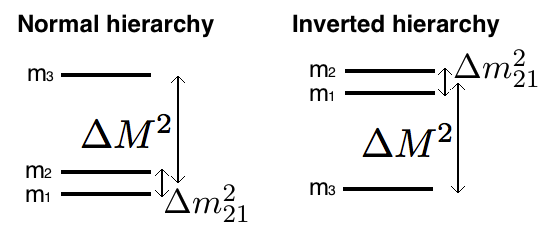
\includegraphics[scale=0.4]{hierarchy_demo.png}
\begin{figure}[h!]
\caption{An illustration of the two possible mass hierarchies, normal (left) is characterised by $m_3$ being larger than $m_1$ and $m_2$, whereas inverted (right) has $m_3$ less than $m_1$ and $m_2$.}
\label{fig:hierarchy_demo}
\end{figure}
\end{center}
\subsubsection{Mixing angles}
The mixing angles describe the amount of each neutrino mass state in each flavour state. They are defined by the following relations\cite{APS}
\begin{align}
\sin^{2}(\theta_{13})= \texttt{ The amount of } \nu_{e} \texttt{ in } \nu_{3},\\
\tan^{2}(\theta_{12})= \frac{\texttt{ The amount of } \nu_{e} \texttt{ in } \nu_{2}}{\texttt{ The amount of } \nu_{e} \texttt{ in } \nu_{3}},\\
\tan^{2}(\theta_{23})= \frac{\texttt{ The amount of } \nu_{\mu} \texttt{ in } \nu_{3} }{\texttt{ The amount of } \nu_{\tau} \texttt{ in } \nu_{3} }.
\end{align}
\subsubsection{CP violation}
If a property of a system remains unchanged when subjected to a spatial transformation, that property is said to be symmetric under that transformation. For example a system that has translational symmetry has a total momentum that is invariant under a translation transformation. In fact our universe appears to be invariant under all translational transformations, which means that momentum is universally conserved. Each conservation law has its own corresponding symmetry and observing which symmetries are broken or conserved can be very informative in physics.\\\\
For a long time the idea of parity conservation was very popular- the theory that the laws of physics would be exactly the same if all spatial coordinates were flipped, like our universe reflected in a mirror. It appeared to be a very good conservation law, being strictly conserved by electromagnetic and strong interactions. However there were a few signs that it might not be conserved in the weak interaction.\\\\
In 1956 Chien-Shiung Wu and colleagues performed an experiment to test parity conservation in the beta decay of cobalt 60 atoms, motivated in part by recent experiments involving kaon decays, which could not be explained if parity was truly conserved. The experiment involved observing the direction in which the beta particle was emitted with respect to a gamma ray, within two mirrored arrangements. The results proved that, in the case of beta decay, parity is not conserved\cite{Wu}.\\\\
It is possible for a system to be symmetric under a combination of transformations, so it was proposed that there must be another transformation that does not form a symmetry on its own, but would do when combined with parity transformation. It was thought that one such transformation could be charge conjugation. This is essentially the transformation of all particles to their respective antiparticles. Charge conjugation symmetry does not appear to hold true in the case of neutrinos, as all neutrinos are observed to have left-handed helicity- their spins point opposite to their momenta, whereas all observed antineutrinos have right-handed helicity. The resulting combination of charge conjugation and parity transformation is called CP symmetry. If CP symmetry holds true, it suggests that a particle and its antiparticle behave exactly the same.\\\\
However CP symmetry is no longer thought to be a fundamental symmetry either, and there is one observation that gives strong justification for this. When the universe formed, matter and antimatter were created in equal proportions, however the universe today is overwhelmingly dominated by matter. When matter and antimatter meet, they annihilate, one-to-one, to produce photons, so there must have been an excess of matter in the early universe for some matter to survive today. The only way such an imbalance could occur is if there is some difference between particles and their antiparticles, in other words CP symmetry is violated.\\\\
There are several instances in the quark sector where CP violation can be observed. There are several instances in the quark sector where CP violation can be observed. The first observation of CP violation was in 1964 when Cronin and Fitch detected the decay of the meson $K_{L}^0$ into two pions at the end of a 57 ft beamline. It was thought that the $K_{L}^0$ could only decay into three pions, as this has the same CP state, but far more two-pion final states were detected than predicted, which indicated CP violation because this final state is not CP symmetric with the initial state\cite{Cronin}. There have since been other observations of CP violation in other kaon decays and with B meson decays.\cite{PDG} So far the amount of CP violation in the quark sector has not been enough to explain the matter-antimatter asymmetry, so the search for CP violation has turned to other areas.\\\\
It is possible that CP symmetry is violated in the lepton sector through a complex phase $\delta_{CP}$, and a major area of interest in neutrino physics is determining the value of this phase. The CP violating phase will manifest itself as a difference in the oscillation probabilities of neutrinos compared to antineutrinos.
\subsection{The PMNS matrix}
The mixing matrix can be thought of as the rotation that transforms the mass state into the flavour state, as in a change of basis.
\begin{centre}
\begin{equation}
\begin{bmatrix}
\nu_{e}\\\nu_{\mu}\\\nu_{\tau}
\end{bmatrix}&=
\begin{bmatrix}
U_{e1}&U_{e2}&U_{e3}\\U_{\mu 1}&U_{\mu 2}&U_{\mu 3}\\U_{\tau 1}&U_{\tau 2}&U_{\tau 3}
\end{bmatrix}
\begin{bmatrix}
\nu_{1}\\\nu_{2}\\\nu_{3}
\end{bmatrix}
\end{equation}}
\end{centre}\\
The three neutrino model requires a three-by-three, unitary matrix, parameterised by the three mixing angles $\theta_{12}$, $\theta_{13}$ and $\theta_{23}$, and the CP violating phase $\delta_{CP}$. The Pontecorvo-Maki-Nakagawa-Sakata or PMNS matrix is the product of three, three-by-three matrices.
\begin{center}
\begin{equation}
U_{\text{{\tiny PMNS}}}=
\underbrace{
\begin{bmatrix}
1&0&0\\0&c_{23}&s_{23}\\0&-s_{23}&c_{23}
\end{bmatrix}
}_\text{atmospheric}
\underbrace{
\begin{bmatrix}
c_{13}&1&s_{13}e^{-i\delta_{CP}}\\0&1&0\\-s_{13}e^{i\delta_{CP}}&0&c_{13}
\end{bmatrix}
}_\text{reactor}
\underbrace{
\begin{bmatrix}
c_{12}&s_{12}&0\\-s_{12}&c_{12}&0\\0&0&1
\end{bmatrix}
}_\text{solar}\\\\
=\begin{bmatrix}
c_{12}c_{13} & s_{12}c_{13} & s_{13}e^{-i\delta_{CP}}\\
-s_{12}c_{23}-c_{12}s_{23}s_{13}e^{i\delta_{CP}} & c_{12}c_{23}-s_{12}s_{23}s_{13}e^{i\delta_{CP}}&s_{23}c_{13}\\
s_{12}s_{23}-c_{12}s_{23}s_{13}e^{i\delta_{CP}} & -c_{12}s{23}-s_{12}c_{23}s_{13}e^{i\delta_{CP}}&c_{23}c_{13}
\end{bmatrix}
\end{equation}
\end{center}
The abbreviations $s_{ij}$ and $c_{ij}$ represent $\sin{\theta_{ij}}$ and $\cos{\theta_{ij}}$ respectively. Current mixing parameter values are based on a global fit of measurements\cite{parameters} from a variety of solar, atmospheric, reactor and accelerator neutrino experiments. They are listed in table \ref{table:parameters}:
\begin{center}
\begin{table}[h]
\centering
    \def\arraystretch{1.5}
    \begin{tabular}{|1|1|}
    \hline
    Parameter & best fit value (\pm1\sigma)\\\hline
    \delta m_{21}^2                   & 7.54_{-0.22}^{+0.26}\times 10^{-5}eV^2 \\\hline
    \Delta M^2 [NH]                   & +2.43_{-0.06}^{+0.06}\times 10^{-3}eV^2\\\hline
        \Delta M^2 [IH]               & -2.38_{-0.06}^{+0.06}\times 10^{-3}eV^2\\\hline
    \sin^2{\theta_{12}}               & 0.308_{-0.017}^{+0.017} \\\hline
    \sin^2{\theta_{23}}, \Delta M^2>1 & 0.437_{-0.023}^{+0.033} \\\hline
    \sin^2{\theta_{23}}, \Delta M^2<1 & 0.455_{-0.031}^{+0.039} \\\hline
    \sin^2{\theta_{13}}, \Delta M^2>1 & 0.0234_{-0.0019}^{+0.0020} \\\hline
    \sin^2{\theta_{13}}, \Delta M^2<1 & 0.0240_{-0.0022}^{+0.0019} \\\hline
    \end{tabular}\\
\caption{Current accepted values for the neutrino mixing parameters, from a global analysis of several neutrino oscillation experiments, as quoted in \cite{parameters}}
\label{table:parameters}
\end{table}
\end{center}\\\\
Figures \ref{fig:electron}, \ref{fig:muon} and \ref{fig:tau} illustrate the three flavour oscillation probabilities for three different starting flavours as functions of $L/E$ at a fixed baseline using the mixing parameters listed in table \ref{table:parameters}.
\begin{center}
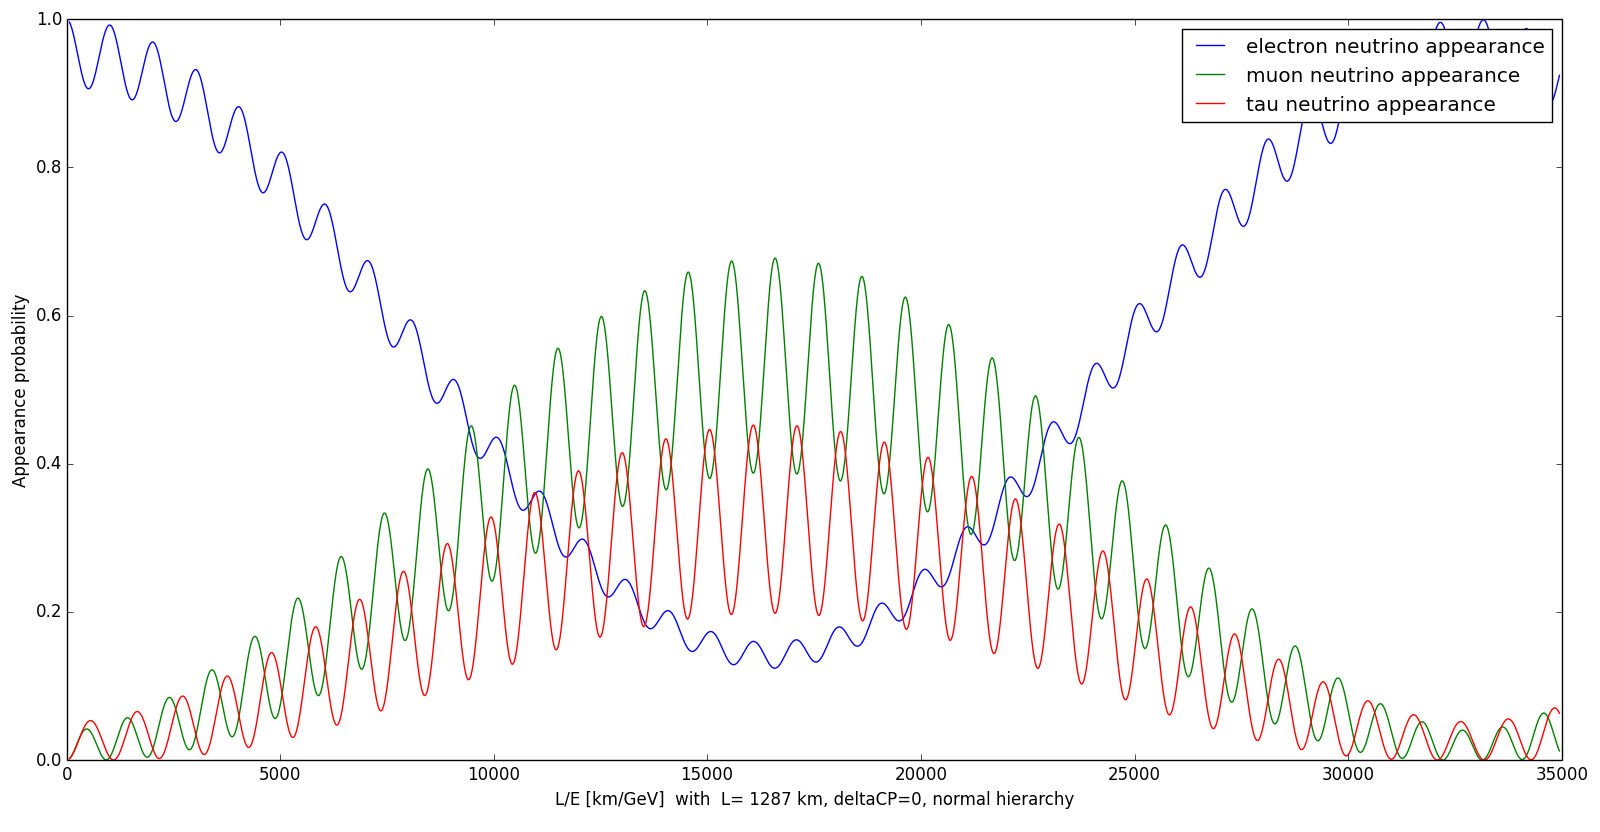
\includegraphics[scale=0.4]{electron_appearance.png}
\begin{figure}[h!]
\caption{Appearance probabilities from an initial electron neutrino.}
\label{fig:electron}
\end{figure}
\end{center}\\\\
\begin{center}
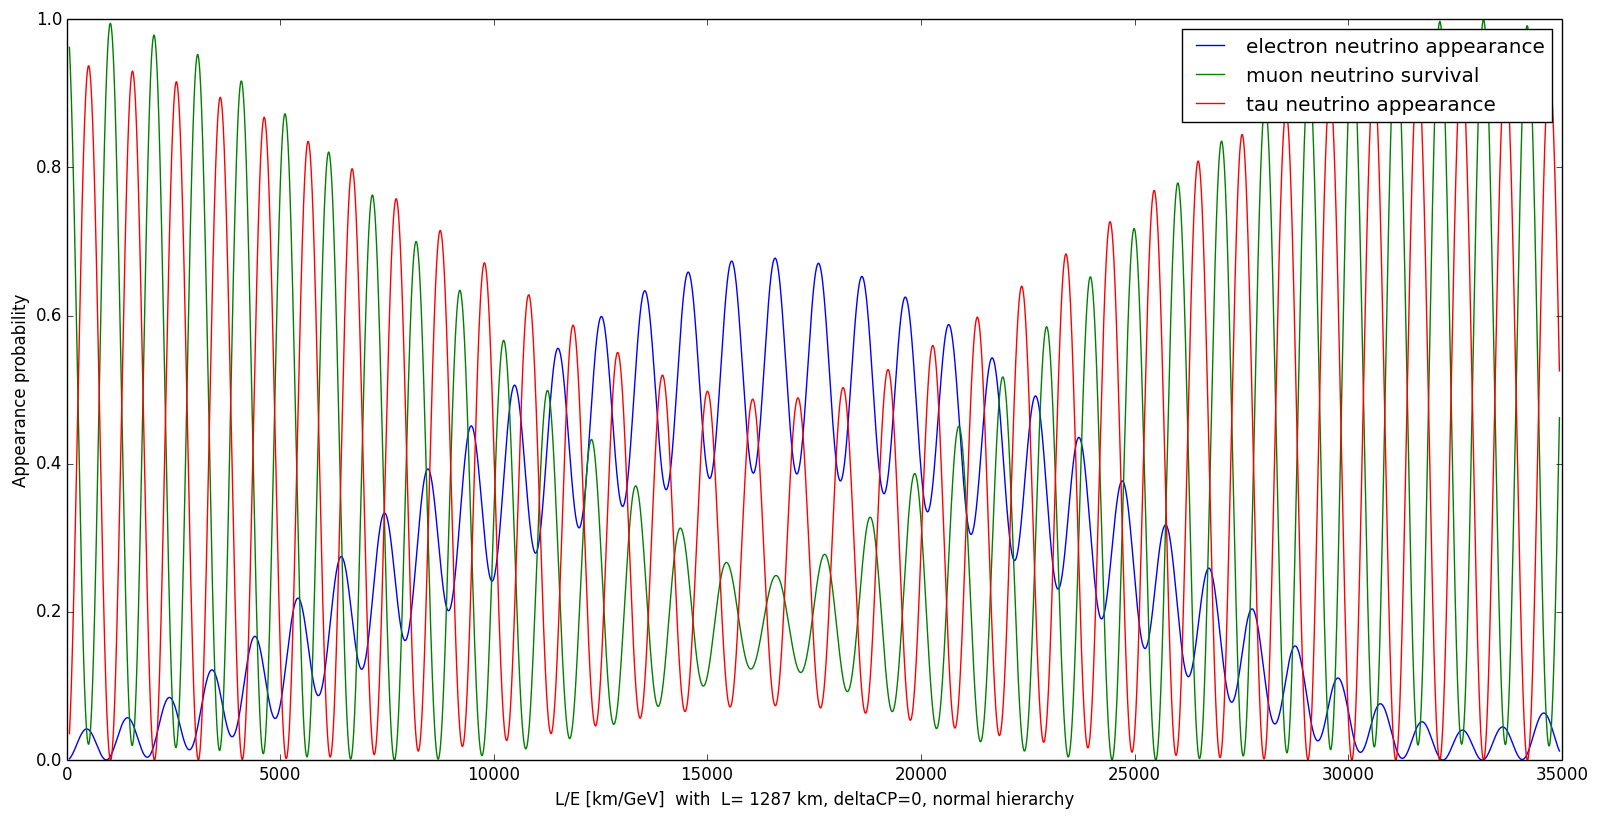
\includegraphics[scale=0.4]{muon_appearance.png}
\begin{figure}[h!]
\caption{Appearance probabilities from an initial muon neutrino.}
\label{fig:muon}
\end{figure}
\end{center}\\\\
\begin{center}
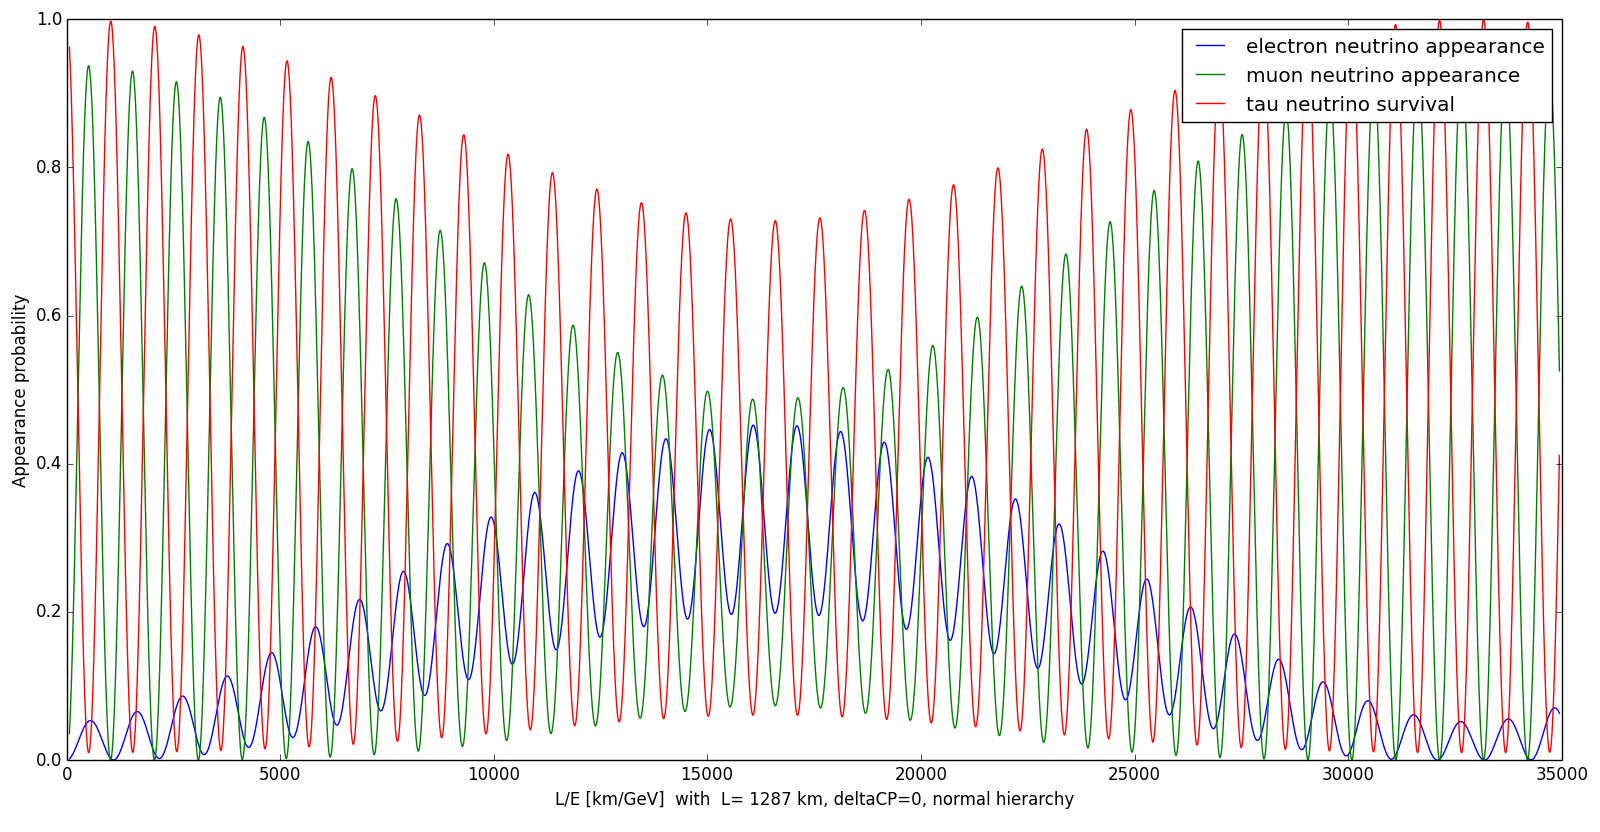
\includegraphics[scale=0.4]{tau_appearance.png}
\begin{figure}[h!]
\caption{Appearance probabilities from an initial tau neutrino.}
\label{fig:tau}
\end{figure}\\\\
\end{center}
Figure \ref{fig:cumulative} shows the flavour state composition of a neutrino as it evolves with $L/E$, starting from a state which is entirely electron flavoured:
\begin{center}
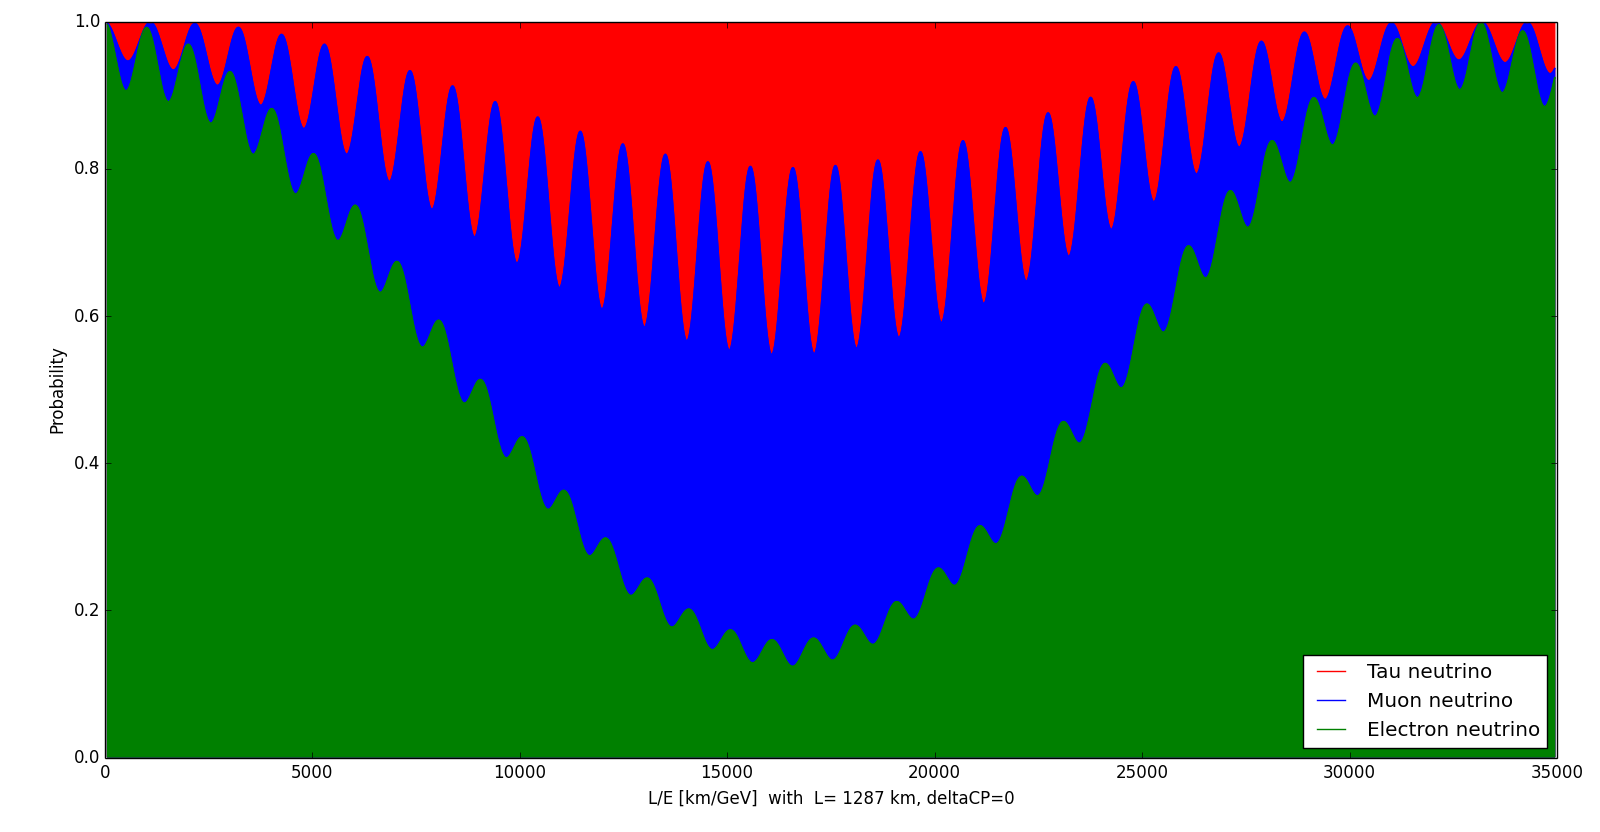
\includegraphics[scale=0.4]{mixing_demo.png}
\begin{figure}[h!]
\caption{Cumulative probabilities for an initial electron neutrino showing its flavour composition as a function of $L/E$.}
\label{fig:cumulative}
\end{figure}\\\\
\end{center}
The small amplitude, `fast' oscillation modes seen in the figures is due to the mixing parameters $\Delta m^2$ , $\theta_{13}$ (referred to as subdominant) and $\theta_{23}$ (referred to as atmospheric), whereas the larger, `slow' oscillation mode is due to the solar mixing parameters- $\Delta m_{12}^2$ and $\theta_{12}$.
\subsection{Matter effects}
Low energies and short baselines are well modelled with vacuum oscillation probabilities, however at higher energies and longer baselines matter effects become very relevant, especially at high matter densities. Certain interactions with the electrons in matter can affect the way different neutrino mass eigenstates propagate, by inducing an effective potential, which ultimately affects their oscillation probabilities. All neutrino flavours are able to scatter off nuclei, but this has a negligible contribution to the matter effect, the main contribution is through elastic forward scattering with electrons\cite{MSW}. Because there are is no $\mu$ or $\tau$ flavoured matter, it is only the electron flavoured component of the mass eigenstate that is affected, as a neutrino can only forward scatter with a lepton with the same flavour. Figure \ref{fig:diagram} shows an electron neutrino forward scattering with an electron.
\begin{center}
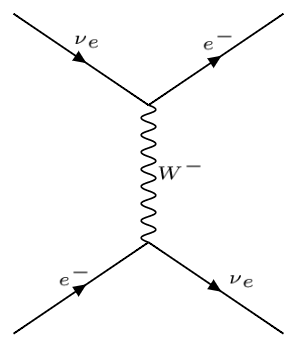
\includegraphics[scale=0.4]{diagram.png}
\begin{figure}[h!]
\caption{An electron neutrino forward scattering off an electron.}
\label{fig:diagram}
\end{figure}
\end{center}\\\\
In a two flavour model the matter effect can be accounted for by introducing an effective mixing angle and mass splitting given by\cite{Zuber}
\begin{align}
\sin(2\theta_m)=&\frac{\sin(2\theta)}{\sqrt{(\frac{\Delta V}{\Delta m^2}-\cos(2\theta))^2+\sin^{2}(2\theta)}},\\
\Delta m_{m}^{2}=&\Delta m^{2}\sqrt{(\frac{\Delta V}{\Delta m^2}-\cos(2\theta))^2+\sin^{2}(2\theta)},\\
\text{where    }\Delta V=&2\sqrt{2}G_{f}EN_{e}
\end{align}
The Fermi interaction constant is represented by $G_f$ and the electron number density is represented by $N_e$. These effective mixing parameters may be substituted into equation \ref{eq:2flavour} to give the corrected two flavour oscillation probability in matter. Figure \ref{fig:2_flavourmatter} shows how a matter density typical of Earth would affect neutrino oscillations.
\begin{center}
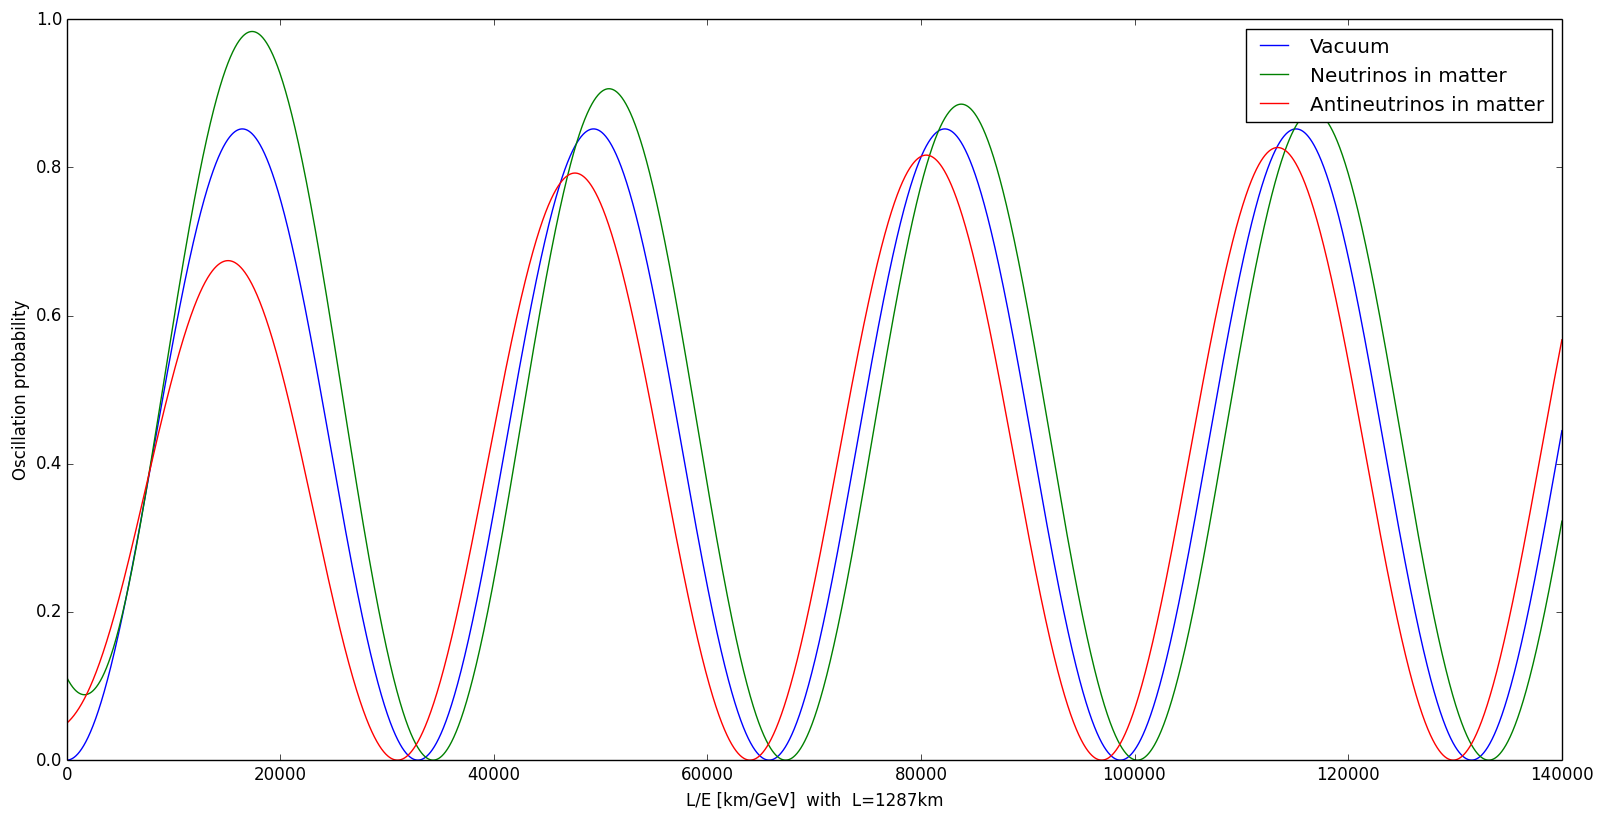
\includegraphics[scale=0.4]{2_flavourmatter.png}
\begin{figure}[h!]
\caption{Electron neutrino (green) and electron antineutrino (red) appearance probabilities in matter from an intial muon neutrino/antineutrino, with a matter density of three times that of water. They are compared to the neutrino/antineutrino appearance probability in vacuum (blue). Oscillations are slowed down for neutrinos and sped up for antineutrinos. The mass hierarchy is normal and $\delta_{CP}=0$.}
\label{fig:2_flavourmatter}
\end{figure}
\end{center}\\\\
Oscillation probabilities for neutrinos in matter are slowed down. For antineutrinos the Fermi constant becomes negative, so matter has the opposite effect on antineutrinos, speeding up their oscillations. This is effectively a CP asymmetry, the system is not CP symmetric because the medium is exclusively made of matter, with no antimatter present.\\\\
The matter effect has been observed in solar neutrinos detected by SNO\cite{SNO}. The effect of solar matter on the propagation of neutrinos is often known as the Mikheyev– Smirnov– Wolfenstein (MSW) effect, which causes electron neutrinos produced in the core of the Sun to propagate in a higher mass eigenstate, which has a smaller `electron-like' component, due to the high density of electrons present in the Sun. The MSW effect has helped to explain the solar neutrino problem, as it causes a more muon neutrinos to be detected on Earth than would otherwise be expected.\\\\
The full three flavour oscillation probability in matter is much more complicated, but can be approximated to first order\cite{analytic} where $\frac{\Delta m_{21}^2}{\Delta m_{31}^2}<<1$ and $\sin^2(\theta_{13})<<1$:
\begin{align}
\label{eq:P}
P_{\nu_{\mu}\rightarrow \nu_{e}}(L,E)\simeq P_0 + P_3 + P_{\sin \delta_{CP}} + P_{\cos \delta_{CP}},
\end{align}
where
\begin{align}
P_0=\sin^2{\theta_{23}}\frac{\sin^2{2\theta_{13}}}{(A-1)^2}\sin^2[(A-1)\Delta],\\
P_3=\alpha^2\cos^2{\theta_{23}}\frac{\sin^2{2\theta_{12}}}{A^2}\sin^2(A\Delta),\\
P_{\sin \delta_{CP}}=\alpha\frac{8J_{CP}}{A(1-A)} \sin{\Delta} \sin{A\Delta}\sin[(1-A)\Delta]\\
P_{\cos \delta_{CP}}=\alpha\frac{8J_{CP}}{A(1-A)} \cos{\Delta} \sin{A \Delta}\sin[(1-A)\Delta],
\end{align}
and
\begin{align}
\alpha = \frac{\Delta m_{21}^2}{\Delta m_{31}^2},\hspace{2mm} \Delta = \frac{\Delta m_{31}^2L}{4E},\hspace{2mm} A=\sqrt{2}G_f N_e \frac{2E}{\Delta m_{31}^2},\\
\label{eq:J}
J_{CP}\equiv Im(U_{\mu 3}U_{e 3}^*U_{e 2}U_{\mu 2}^2)=\frac{1}{8}\cos \theta_{13}\sin 2\theta_{12}\sin 2\theta_{23}\sin 2\theta_{13}\sin \delta_{CP}.
\end{align}
`$J_{CP}$' is known as the Jarlskog Invariant. It carries the CP phase dependence and becomes negative for antineutrinos. The `$A$' carries the matter effect and also changes sign for antineutrinos, but will also change sign if the hierarchy is inverted, because as $\Delta m_{31}^2$ will be negative, so for antineutrinos and inverted hierarchy it will be positive again. `$\Delta$' carries the mass hierarchy dependence by being positive for normal hierarchy and negative for inverted hierarchy. The matter effect and CP phase can combine in different ways, so for certain mater densities and CP phases the effects completely cancel out. Figure \ref{fig:CP} illustrates the effect of the CP phase on the first few oscillation maxima, by showing $\nu_e$ and $\overline{\nu}_e$ appearance probabilities from an initial $\nu_{\mu}$ and $\overline{\nu}_{\mu}$ with a CP violating phase of $\pi/2$.
\begin{center}
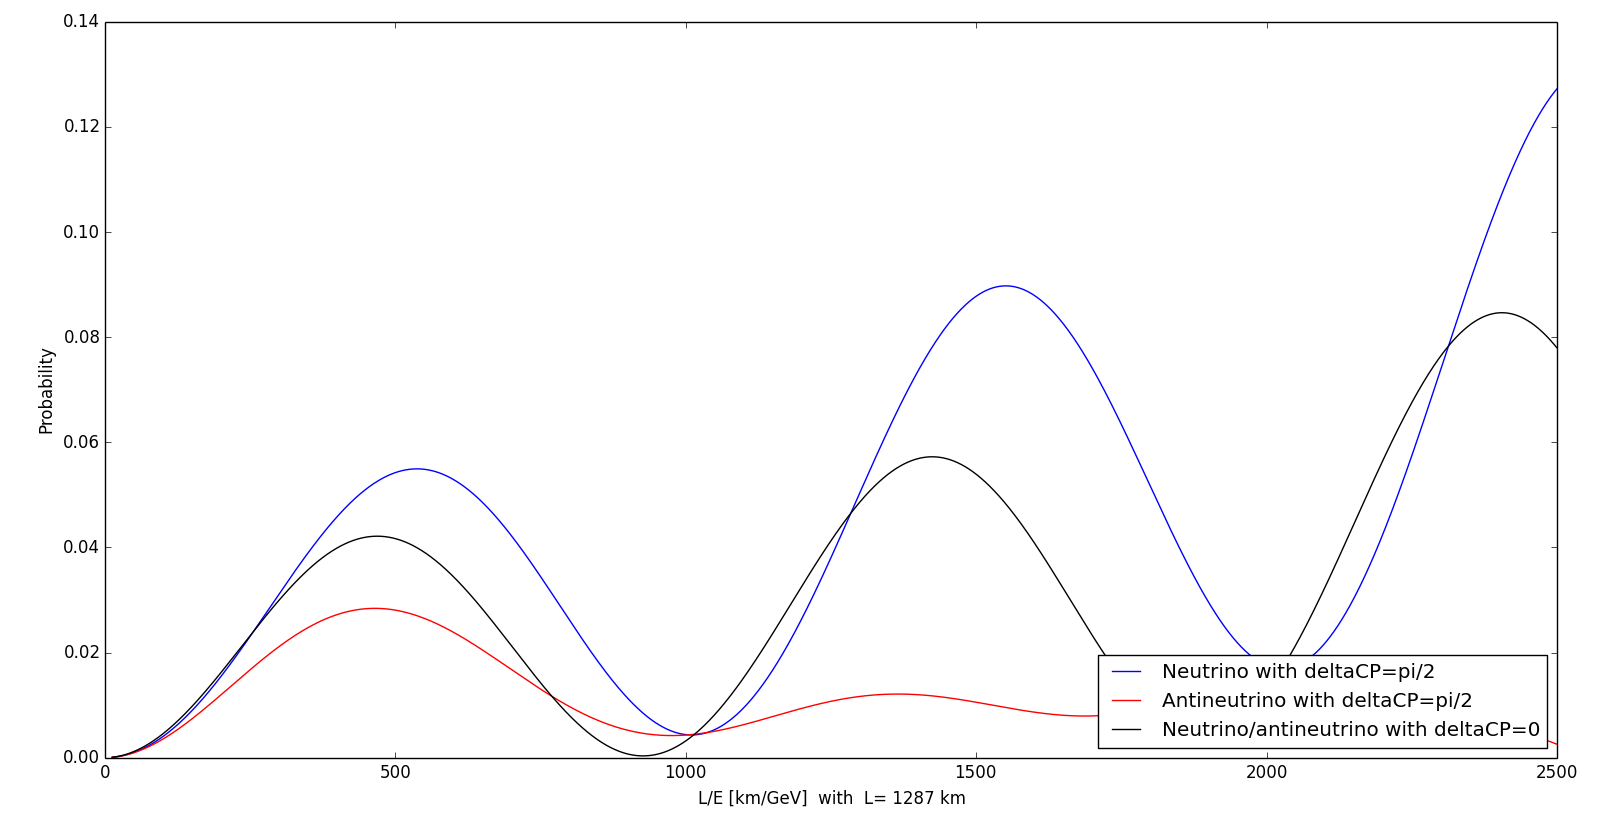
\includegraphics[scale=0.4]{CP_effect.png}
\begin{figure}[h!]
\caption{Appearance probabilities for an electron neutrino/antineutrino (blue/red) from an initial muon neutrino and antineutrino with $\delta_{CP}=\pi/2$ to show the effect of the CP phase. They are compared with the case where $\delta_{CP}=0$ (black). The mass hierarchy is normal.}
\label{fig:CP}
\end{figure}
\end{center}\\\\
Figure \ref{fig:matter} shows the effect of matter on oscillations by showing the appearance probabilities for $\nu_{e}$ and $\overline{\nu}_{e}$ in matter and also in vacuum with no CP phase (appearance probabilities are the same for neutrinos and antineutrinos in vacuum). The amplitude and period of oscillation are increased for neutrinos, and decreased for antineutrinos.
\begin{center}
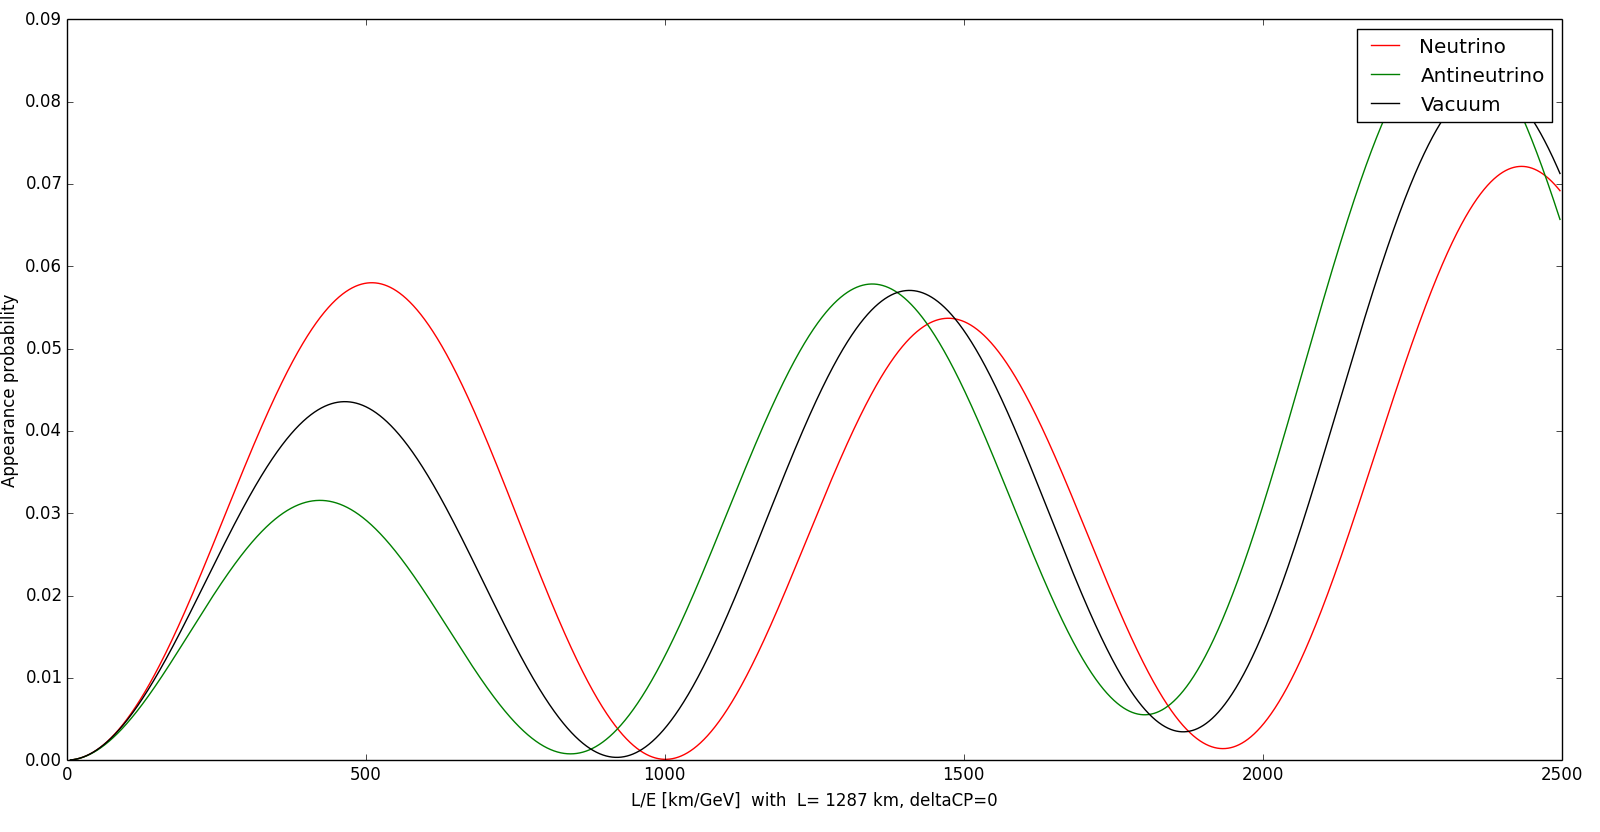
\includegraphics[scale=0.4]{matter_effect.png}
\begin{figure}[h!]
\caption{Appearance probabilities for an electron neutrino/antineutrino (red/green) from an initial muon neutrino/antineutrino with a matter density of twice that of water, showing the effect of matter. The appearance probability for the vacuum case is also shown (black). The mass hierarchy is normal with $\delta_{CP}=0$.}
\label{fig:matter}
\end{figure}
\end{center}\\\\
Figure \ref{fig:MH} shows what effect the mass hierarchy would have on electron neutrino appearance probabilities for an initial muon neutrino. The difference between mass hierarchies is subtle, but combined with the matter effect over a long baseline the difference can be enhanced, as shown in figure \ref{fig:MHinmatter}.
\begin{center}
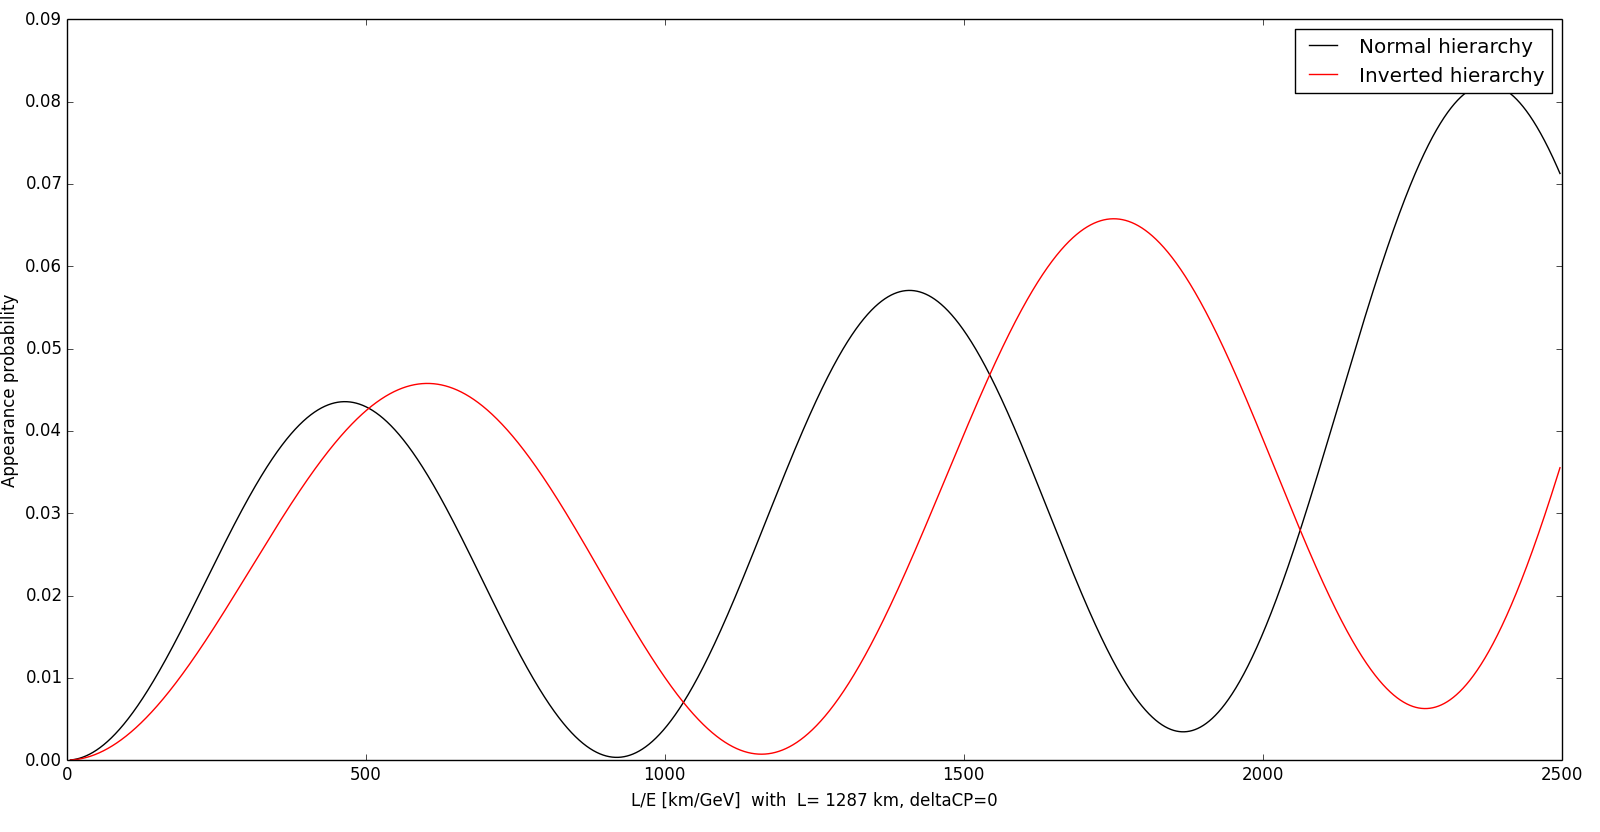
\includegraphics[scale=0.4]{hierarchy_effect.png}
\begin{figure}[h!]
\caption{Appearance probabilities for electron neutrinos from an initial muon neutrino, with normal hierarchy (black) and inverted hierarchy (red). $\delta_{CP}=0$ there is no matter effect.}
\label{fig:MH}
\end{figure}
\end{center}\\\\
\begin{center}
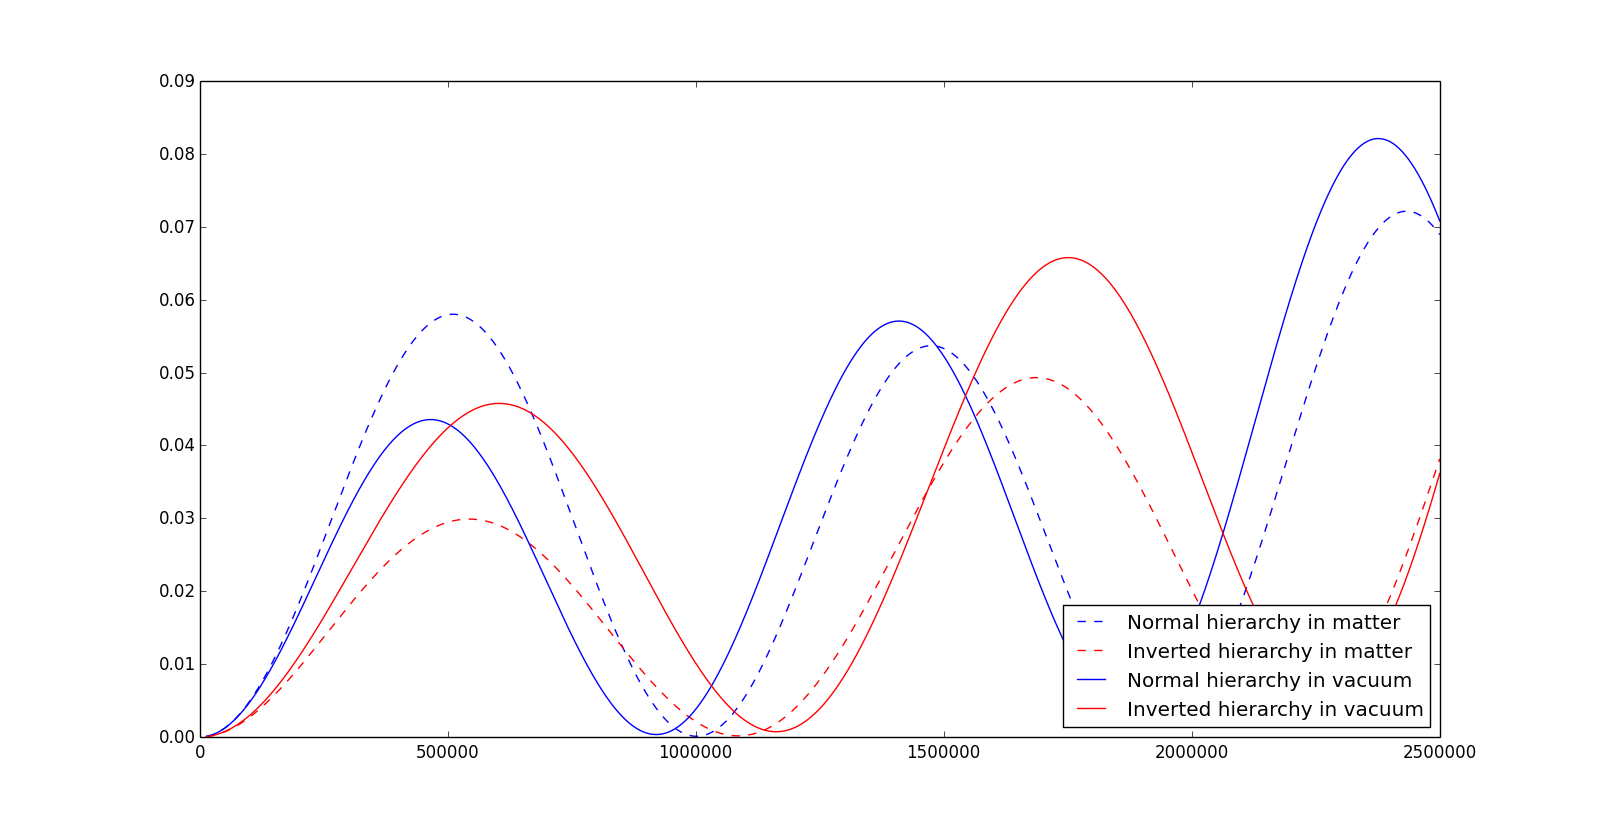
\includegraphics[scale=0.4]{MH_in_matter.png}
\begin{figure}[h!]
\caption{Appearance probabilities for an electron neutrino from an initial muon neutrino in matter (dashed) and in vacuum (solid) with normal hierarchy (blue) and inverted hierarchy (red). $\delta_{CP}=0$ and the density used is twice that of water.}
\label{fig:MHinmatter}
\end{figure}
\end{center}
\subsection{Existing neutrino oscillation experiments}
\subsubsection{Existing types of neutrino source}
There are four main sources of neutrinos that are used for experiments; atmospheric, solar, reactor and accelerator. Because each source type has its own unique energy spectrum, they are all very useful for learning about neutrinos, and our knowledge of the PMNS matrix parameters as they stand today are informed by a wide range of neutrino experiments.\\\\
Atmospheric neutrinos are produced when cosmic rays, typically high energy protons, hit nuclei in the Earth's upper atmosphere. The resulting hadronic showers produce many charged mesons, which subsequently decay to produce muon and electron neutrinos. Because of the high energies of the incident cosmic rays, atmospheric neutrinos can have enormous energies, sometimes in the range of TeV\cite{Zuber}. Super-Kamiokande is a neutrino detector in Kamioka, Japan, which produced some of the first evidence for neutrino oscillation in 1998 by observing a difference in the atmospheric muon neutrino flux coming from the downwards direction and the upwards direction (i.e. through the Earth). In the absence of oscillations there should be no muon neutrino flux difference, but due to the neutrinos travelling a longer distance, they were able to oscillate into other flavours that were not detectable by the experiment\cite{SuperK}. Atmospheric neutrino experiments are most sensitive to $\theta_{23}$ and $\Delta M^2$, known as the atmospheric oscillation parameters.\\\\
Solar neutrinos dominate the neutrino flux on Earth and are produced by nuclear fusion reactions in the Sun's core, with an energy range of a few hundred KeV to roughly 20 MeV. Solar neutrinos have been used to study the fusion processes in the Sun, and produced the first clue that neutrinos might oscillate, in Davis and Bahcall's famous Homestake experiment. In 2001 the Sudbury Neutrino Observatory (SNO) in Canada, published conclusive evidence of neutrino oscillation as well as measurements the total electron neutrino flux, by observing total solar neutrino fluxes, which also helped to consolidate the Standard Solar Model\cite{SNO1}. Solar neutrino experiments are most sensitive to $\theta_{12}$ and $\Delta m_{21}^2$, known as the solar oscillation parameters.\\\\
Reactor neutrinos are the by-products of nuclear fission in reactors and have a typical energy range of just a few MeV\cite{reactor}. An advantage of reactor experiments is the ability to control the neutrino flux produced, and build a detector close to the source, allowing one to make measurements at the source, and again at a far detector, which is very useful in oscillation experiments as the exact change in flux can be inferred. The Daya Bay experiment in China produced the first non-zero measurement of $\theta_{13}$ using reactor neutrinos\cite{Daya}. This last mixing angle is sometimes referred to as the sub-dominant angle.\\\\
Accelerator neutrinos are the most recent front of neutrino research. Accelerator neutrinos are produced by high energy particle beams in colliders, which are aimed at stationary targets, producing (among other things) charged mesons, which are then allowed to decay into leptons. Accelerators can produce neutrinos with energies of up to roughly 20 GeV with very high intensity\cite{accelerator}. They can produce neutrinos in collimated beams, which can be directed towards a detector. This means that an accelerator neutrino experiment can have a very long baseline compared to a reactor experiment without losing too much intensity. The NuMI Off-Axis $\nu_e$ Appearance (NOvA) experiment is a current experiment which sends a beam of muon neutrinos over a distance of roughly 800 km from Fermilab in Illinois, to a detector in Minnesota, in order to determine the true neutrino mass hierarchy\cite{NOvA}.
\subsubsection{Existing types of detector}
The biggest challenge faced by neutrino experiments is detection, as neutrinos interact so rarely. There are only two types of interaction that neutrinos take part in: Neutral Current (NC) and Charged Current (CC). In a CC interaction an incident neutrino exchanges a $W^{\pm}$ boson with another particle, to become a charged lepton, as shown in figure \ref{fig:CC}. The flavour and energy of the incident neutrino can be inferred by detecting the charged lepton produced. The neutrino must have enough energy to produce its corresponding charged lepton, CC events are more common for electron neutrinos, and much rarer for tau neutrinos. In a NC event a neutrino exchanges momentum with another particle by the exchange of a neutral $Z^0$ boson as shown in figure \ref{fig:NC}. An upper limit on the energy of the incident neutrino can be inferred, but it is not possible to infer its flavour. Neutrino detectors exploit CC and NC interactions to gain as much information as possible about the neutrinos that pass through them.\\\\
\begin{center}
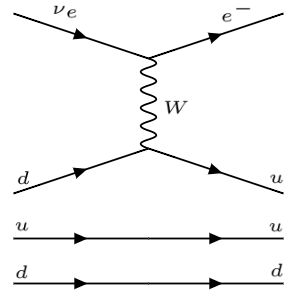
\includegraphics[scale=0.4]{CC.png}
\begin{figure}[h!]
\caption{An electron neutrino exchanging a $W^+$ boson with a neutron (left) by exchanging a $W^+$ boson in a CC interaction, producing an electron and a proton (right).}
\label{fig:CC}
\end{figure}
\end{center}
\begin{center}
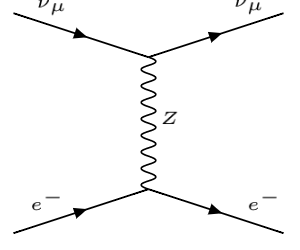
\includegraphics[scale=0.4]{NC.png}
\begin{figure}[h!]
\caption{A muon neutrino scattering off an electron by exchanging a neutral $Z^0$ boson.}
\label{fig:NC}
\end{figure}
\end{center}
The detector used by Davis and Bahcall in the Homestake experiment was a chlorine detector. This consisted of a large tank filled with tetrachloroethylene, which is fluid that contains chlorine atoms. Neutrinos hit the nuclei of a chlorine-37 isotopes, and via CC interactions, causing neutrons to turn into protons, creating Argon-37 nuclei. By counting how many radioactive Argon-37 isotopes were present in the tank, the number of neutrino interaction events could be calculated\cite{Homestake}. The minimum energy a neutrino must have to be detected in this way is roughly 0.8 MeV, although other isotopes can also be used, which have lower energy thresholds, such as Gallium-71. This method does not allow the neutrino energy to be measured, but it is very useful for measuring total flux.\\\\
Cherenkov detectors detect the products of CC interactions as they move at relativistic speeds through a medium. Cherenkov radiation is emitted when a particle moves through a medium with a speed higher than the speed of light in that medium. As the particle travels, it causes an electromagnetic `shock-wave', analagous to a sonic boom produced by a body moving faster than the speed of sound. This electromagnetic The Cherenkov `shock-wave' propagates in a conical shape centered around the particle. A Cherenkov detector consists of a large volume of some medium, for example water, surrounded by an array of Photo-Multiplier Tubes (PMTs) mounted to the container walls. The PMTs detect the Cherenkov radiation from relativistic particles, which will cast rings of light on the walls of the detector. The characteristics of these rings can be used to infer what type of particle caused them, including their energy and flavour\cite{leo}. Cherenkov detectors typically detect the muons and electrons that result from neutrino interactions. Many neutrino experiments use Cherenkov detectors, including SNO and Super-Kamoikande.\\\\
A Time Projection Chamber (TPC) is a type of detector which measures the ionisation caused by charged particles travelling through its medium. The ionisation electrons are detected after being drifted towards anodes. The position of the ionisation event within the drift volume can be inferred by the time taken for the electron to drift to the anode\cite{leo}. TPCs allow very precise measurement of energy too, because the amount of ionisation caused by a particle is related to its momentum. Unless it is magnetised, a TPC cannot distuinguish between neutrino and antineutrino events. An example of a TPC is the one used by the Imaging Comsic And Rare Underground Signals experiment, which uses a 600 ton liquid argon TPC\cite{ICARUS}. 
\section{The Long Baseline Neutrino Experiment}
\subsection{Aims of the Long Baseline Neutrino Experiment}
The Long Baseline Neutrino Experiment (LBNE) is an international scientific collaboration designed primarily to determine the neutrino mass hierarchy and measure the CP violating phase. LBNE will consist of a high purity muon neutrino beam produced at the Fermilab facility in Batavia, Illinois, passing through a near detector and directed at a detector 1300 km away at Homestake Mine in Lead, South Dakota. The beam will pass underground through the Earth's crust. The baseline and energy range of the experiment are chosen so that sensitivity to oscillation effects will be maximised. LBNE will also refine the current measurements of oscillation parameters such as $\theta_{13}$ and $\Delta m_{32}^2$\cite{LBNE}. LBNE has recently changed its name to Deep Underground Neutrino Experiment (DUNE).
\subsection{The beamline}
The beam will be produced by the Neutrinos at the Main Injector (NuMI) facility at Fermilab, the same one used by the Main Injector Neutrino Oscillation Search (MINOS) \cite{MINOS} and currently used by the Off-axis $\nu_e$ Appearance (NOvA) project\cite{NOvA}. A High intensity proton beam will be extracted from the Main Injector accelerator and directed towards a graphite target, to produce a beam of pions and kaons. These will be directed by magnetic focusing horns to a decay pipe filled with helium, where they will decay to muons and muon neutrinos.\\\\
The magnetic focusing horn polarity can be changed to favour neutrinos or antineutrinos, and the graphite target can be positioned in different ways relative to the focusing horns to give different energy spectra. So there are several possible beam energies and polarities. This project will consider the Low Energy beam tuning, where the target is located 35cm from the first focusing horn, alternately running on both horn polarities to produce a neutrino-dominant or antineutrino-dominant beam with an energy spectrum ranging from 0.5 GeV to 20 GeV\cite{LBNE}. This energy range will include the first and second oscillation maxima for the baseline of 1300km. It is assumed that the Main Injector accelerator will deliver a total of $1.5\times 10^{21}$ Protons On Target (POT) per year and will run for equal times with each focusing horn polarity.
\subsection{The near detector}
The near detector must measure to a high precision the unoscillated flux of $\nu_{\mu}$, $\overline{\nu}_{\mu}$, $\nu_{e}$ and $\overline{\nu}_{e}$, in order to understand the signal background and allow measurement of $\nu_{\mu}/\overline{\nu}_{\mu}$ disappearance. The near detector will be magnetised to discriminate between neutrino and antineutrino events, and will be located roughly 500 m from the target so oscillation will be negligible at this stage. The $\nu_{e}/\overline{\nu}_{e}$ components of the beam are expected to be small compared to the $\nu_{\mu}/\overline{\nu}_{\mu}$ components and so are neglected in this project. Figures \ref{fig:spectrum1} and \ref{fig:spectrum2} show the $\nu_{\mu}$ and $\overline{\nu}_{\mu}$ components of the beam flux expected at 1300km, per GeV proton beam energy, per $10^{20}$ POT \cite{LBNE}:
\begin{center}
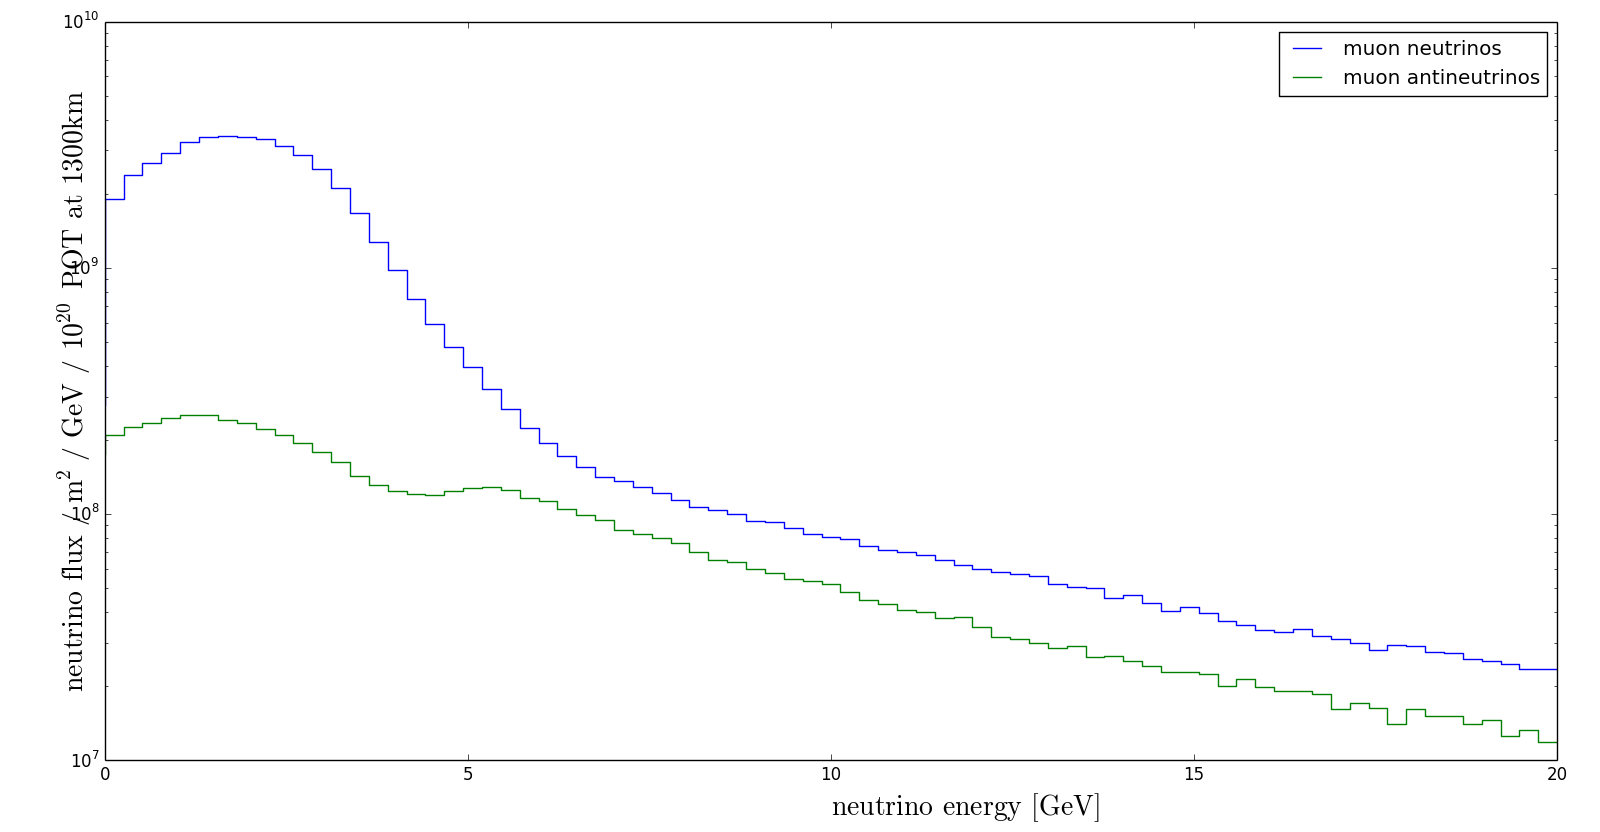
\includegraphics[scale=0.4]{neutrino_beam.png}
\begin{figure}[h!]
\caption{The simulated, unoscillated energy spectrum for the low energy beam tuning in the neutrino-dominant mode at 1300 km. Electron neutrinos/antineutrinos are neglected. The data is taken from \cite{LBNE}.}
\label{fig:spectrum1}
\end{figure}
\end{center}\\\\
\begin{center}
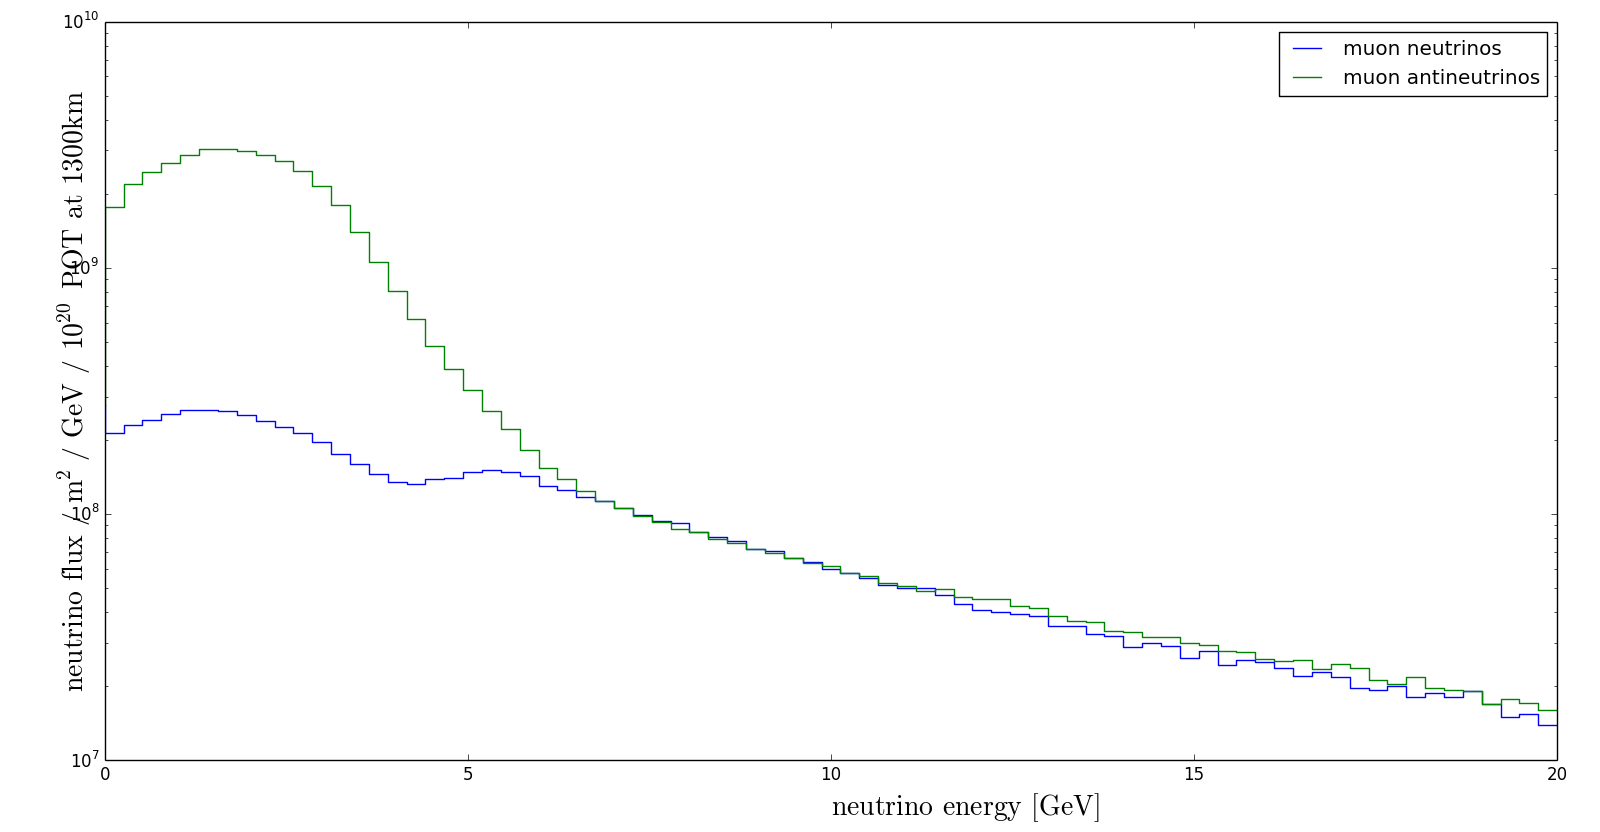
\includegraphics[scale=0.4]{antineutrino_beam.png}
\begin{figure}[h!]
\caption{The simulated, unoscillated energy spectrum for the low energy beam tuning in the antineutrino-dominant mode at 1300 km. Electron neutrinos/antineutrinos are neglected. The data is taken from \cite{LBNE}}
\label{fig:spectrum2}
\end{figure}
\end{center}
\subsection{The far detector}
The far detector will be a Liquid Argon Time Projection Chamber  (LArTPC) located nearly 5000 ft underground, which will be able to distinguish between $\nu_{\mu}/\overline{\nu}_{\mu}$ and $\nu_{e}/\overline{\nu}_{e}$ events and measure their energies with high precision. The beam can be selected to produce mostly neutrinos or mostly antineutrinos, but the far detector will not be magnetised so it cannot distinguish between neutrino and antineutrino events\cite{LBNE}.\\\\
The LArTPC will consist of an assembly of wire planes arranged in such a way that the position of each event can be precisely inferred by the signal induced in each wire, due to the drifting ionisation electrons. The medium will be liquid argon, chosen for its stability and relative abundance, as well as other properties such as its density and scintillation wavelength. The final stage design for the LBNE far detector will have a 50kt volume of liquid argon.
\subsection{Determining the mass hierarchy and CP phase}
Methods used by the author to predict the sensitivity that might be achieved by the LBNE are outlined in this section.

Using the methods shown in equations (\ref{eq:P}) to (\ref{eq:J}), the appearance probabilities for each energy bin shown in figures \ref{fig:spectrum1} and \ref{fig:spectrum2} can be multiplied by the total flux expected in that energy bin, to give the oscillated spectrum\cite{LBNE}. In this project the interaction cross-section for CC events is approximated to be constant with energy, and statistical and detector effects are neglected. The expected oscillated energy spectrum for $\nu_e / \overline{\nu}_e$ appearance events at a 50kt far detector exposed to either the neutrino or antineutrino beam mode is shown in figure \ref{fig:signal}. The total number of events is scaled to match the expected number of $\nu_e / \overline{\nu}_e$ CC events obtained from a simulation\cite{GLOBES}, for a detector mass of 50kt at 1300km, running for one year, with the beam running at 1.2 MW, at an energy of 80 GeV, producing $1.5\times 10^{21}$ POT per year. The density of the beam path is taken to be twice that of water\cite{PREM}.
\begin{center}
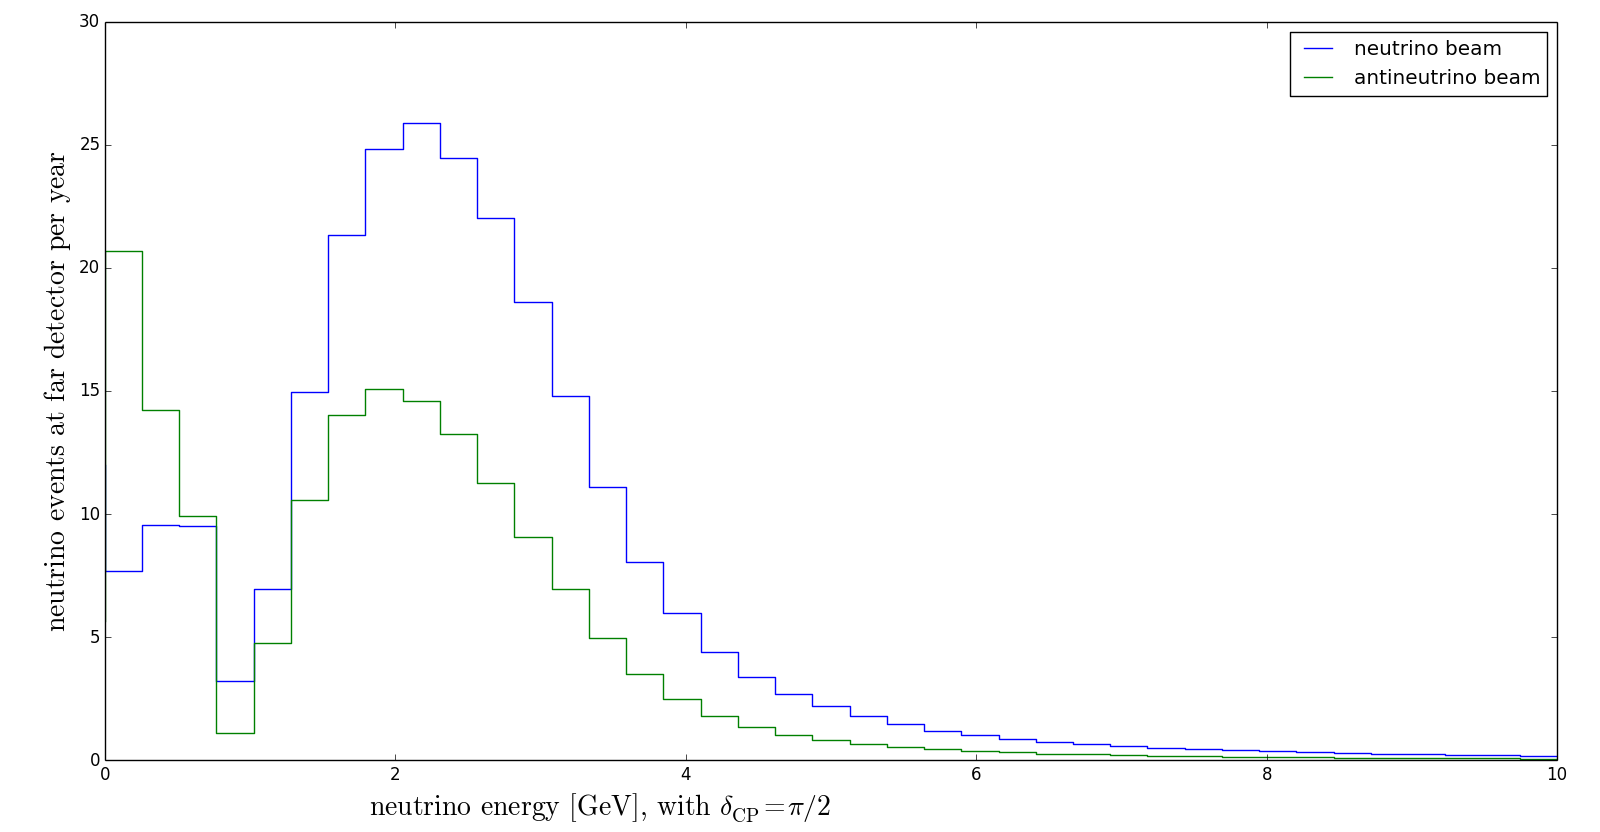
\includegraphics[scale=0.4]{Signal.png}
\begin{figure}[h!]
\caption{Far detector signal for a 50kt LArTPC with zero CP phase and normal hierarchy. No statistical or detector effects are included, with CC cross-sections approximated as being constant with energy. The proton beam is assumed to be running at 1.2 MW, at 80GeV, producing $1.5\times 10^{21}$ POT per year, for 1 year.}
\label{fig:signal}
\end{figure}
\end{center}
The position and amplitude of the main peak visible in figure \ref{fig:signal} are functions of the true CP violating phase and the true mass hierarchy, so by observing this signal and comparing it with the three flavour model described in equations (\ref{eq:P}) to (\ref{eq:J}) the true values of these can be determined. To discriminate between two different hypotheses, the quantity $\Delta \chi^2$ is calculated. It is defined as the difference between the $\chi^2$ values of the two hypotheses. When determining the true mass hierarchy the value of $\Delta \chi^2_{MH}$ is calculated as the difference between the $\chi^2$ of the true signal versus that of a predicted signal with the mass hierarchy being tested. This is how $\chi^2$ and $\Delta \chi^2$ are calculated when determining the mass hierarchy\cite{CHI}:
\begin{align}
\chi^2(n^{true},n^{test})=2\sum\limits_{i}^{N}(n_{i}^{true})\ln{\frac{n_{i}^{true}}{n_{i}^{test}}},\\
\Delta \chi^2_{MH}=|\chi^2_{test=IH}-\chi^2_{test=NH}+s_{i}^{test}-s_{i}^{true}|,
\end{align}
where the summation is over all signal energy bins and $n_i$ is the number of events in that bin. The sensitivity of the experiment is quantified by $\sqrt{\Delta \chi^2}$. This is illustrated as a function of the true CP violating phase for both possible true mass hierarchies in figure \ref{fig:sensitivity1}. The calculated signals used for the figures do not take into account statistical or detector effects so the sensitivity is that of a perfect experiment, and therefore slightly inflated. The shape of the curve in figure \ref{fig:sensitivity1} is expected to be roughly sinusoidal\cite{LBNE}, but the the Earth's density profile has been approximated as constant, which does not fully account for the matter effect. This should not have a significant effect on the sensitivity to CP violation.
\begin{center}
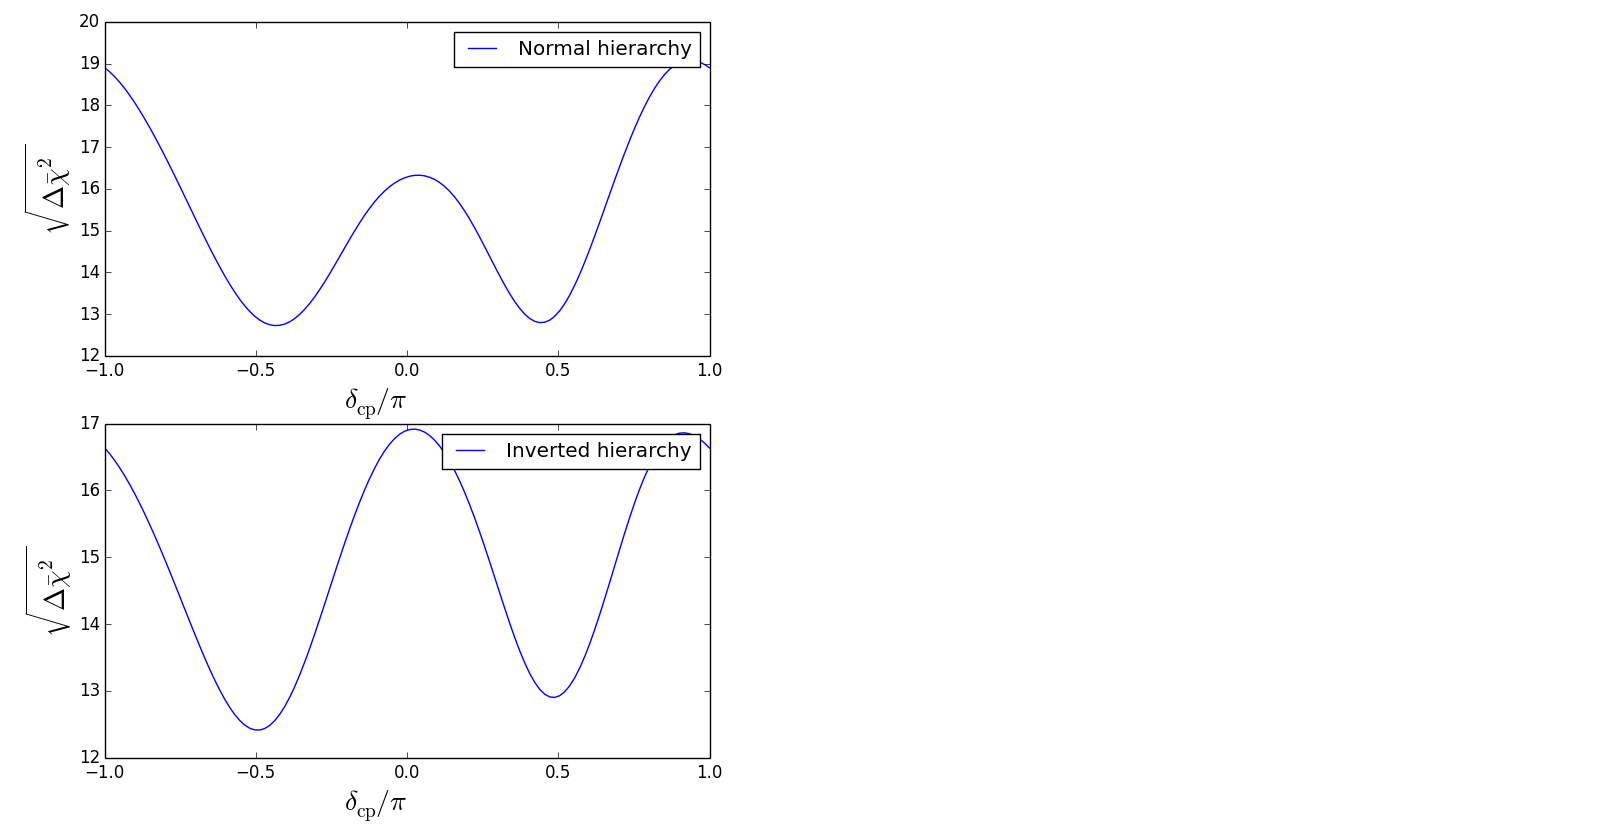
\includegraphics[scale=0.9]{MH_sensitivity.png}
\begin{figure}[h!]
\caption{Sensitivity to the mass hierarchy as a function of $\delta_{CP}$ for the cases where true mass hierarchy is normal (top) or inverted (bottom). Assumptions are a 1.2 MW, 80 GeV proton beam producing $1.5\times 10^{21}$ POT per year, running for 1 year, with a 50 kt detector mass.}
\label{fig:sensitivity1}
\end{figure}
\end{center}
The same approach is taken to predict the sensitivity of the LBNE to CP violation. CP violation would be characterised by the true CP phase having any value but $0$ or $\pi$. In this case $\Delta \chi^2$ is given by \cite{CHI}
\begin{align}
\Delta \chi^2_{CP}=\chi_{\delta_{CP}^{test}}^{2}-\chi_{\delta_{CP}^{true}}^{2},\\
\Delta \chi^2_{CPV}=\text{min}(\chi^2_{CP}(\delta_{CP}^{test}=0),\chi^2_{CP}(\delta_{CP}^{test}=\pi)).
\end{align}
The sensitivity to CP violation as a function of the true CP phase is shown in figure \ref{fig:sensitivity2}. The CP violating component of the appearance probability is sinusoidal in $\delta_{CP}$, so it is expected that the maximum sensitivity to CP violation should occur for near the true CP phase values of $\pm\pi/2$, which is indeed what is seen in figure \ref{fig:sensitivity2}.
\begin{center}
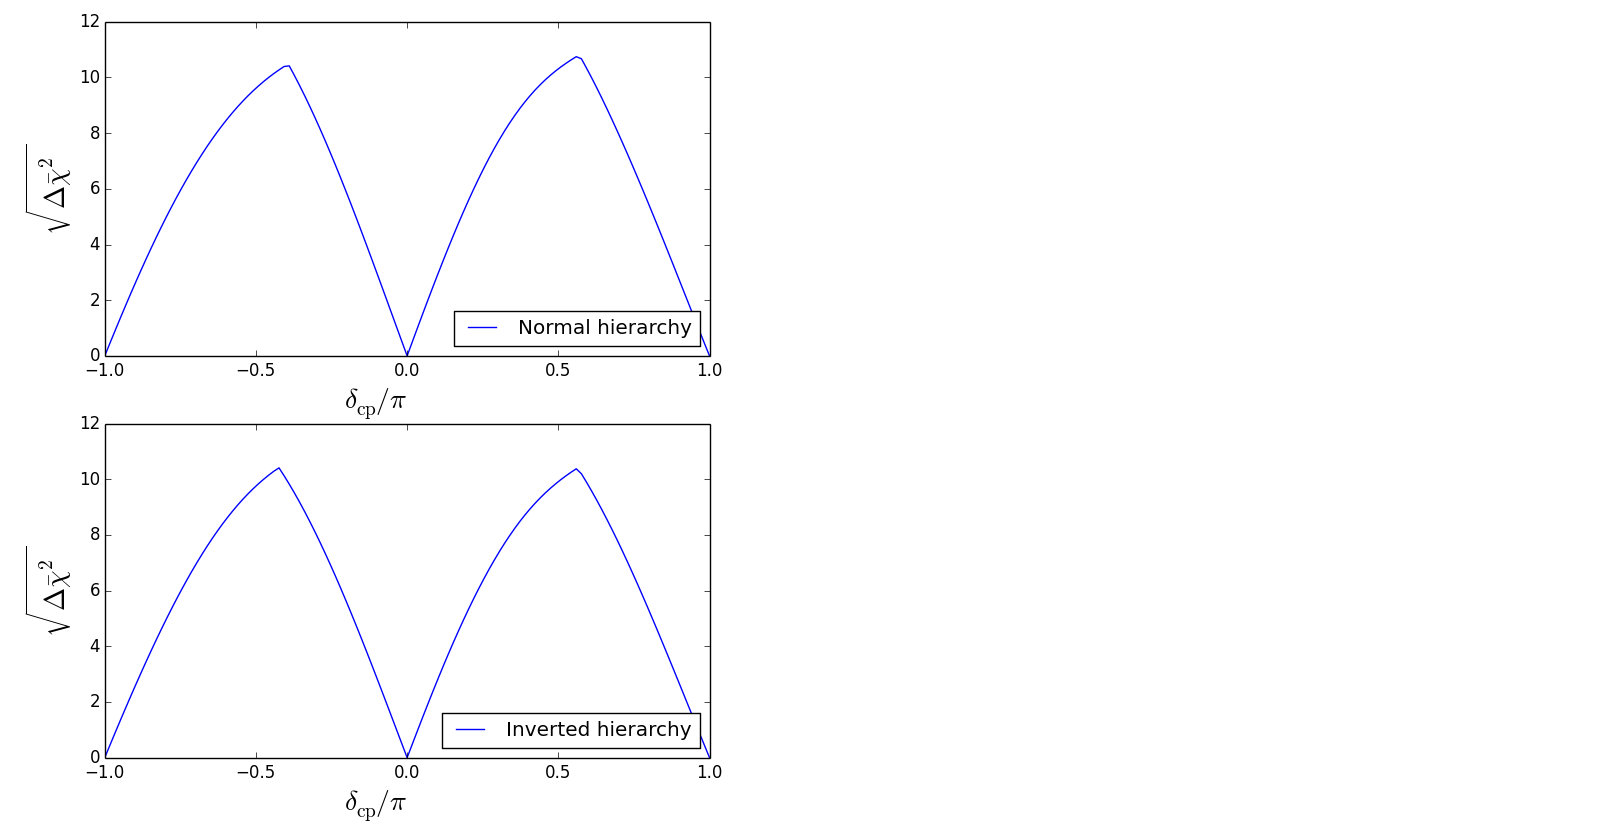
\includegraphics[scale=0.9]{CPV_sensitivity.png}
\begin{figure}[h!]
\caption{Sensitivity to CP violation as a function of $\delta_{CP}$ for both mass hierarchies. Assumptions are a 1.2 MW, 80 GeV proton beam producing $1.5\times 10^{21}$ POT per year, running for 1 year, with a 50 kt detector mass.}
\label{fig:sensitivity2}
\end{figure}
\end{center}\\\\
In reality, LBNE may not receive the full funding requested, so a 50 kt LArTPC may not be a realistic scenario. The detector may instead have a mass of 10 kt, which would decrease the sensitivity of the experiment to CP violation and the true mass hierarchy. Figures \ref{fig:sensitivity4} and  \ref{fig:sensitivity3} show the sensitivities to the true mass hierarchy and CP violation that can be achieved with the same assumptions as in figure \ref{fig:sensitivity2}, but with a 10 kt LArTPC instead of 50 kt. In both case the sensitivity is roughly halved, although it may still be possible to determine the true mass hierarchy with an acceptable level of confidence. It is possible to compensate for the lower sensitivity with a longer exposure time, i.e. running the experiment for a longer time period. This would be achieved by running the experiment for five times as long.
\begin{center}
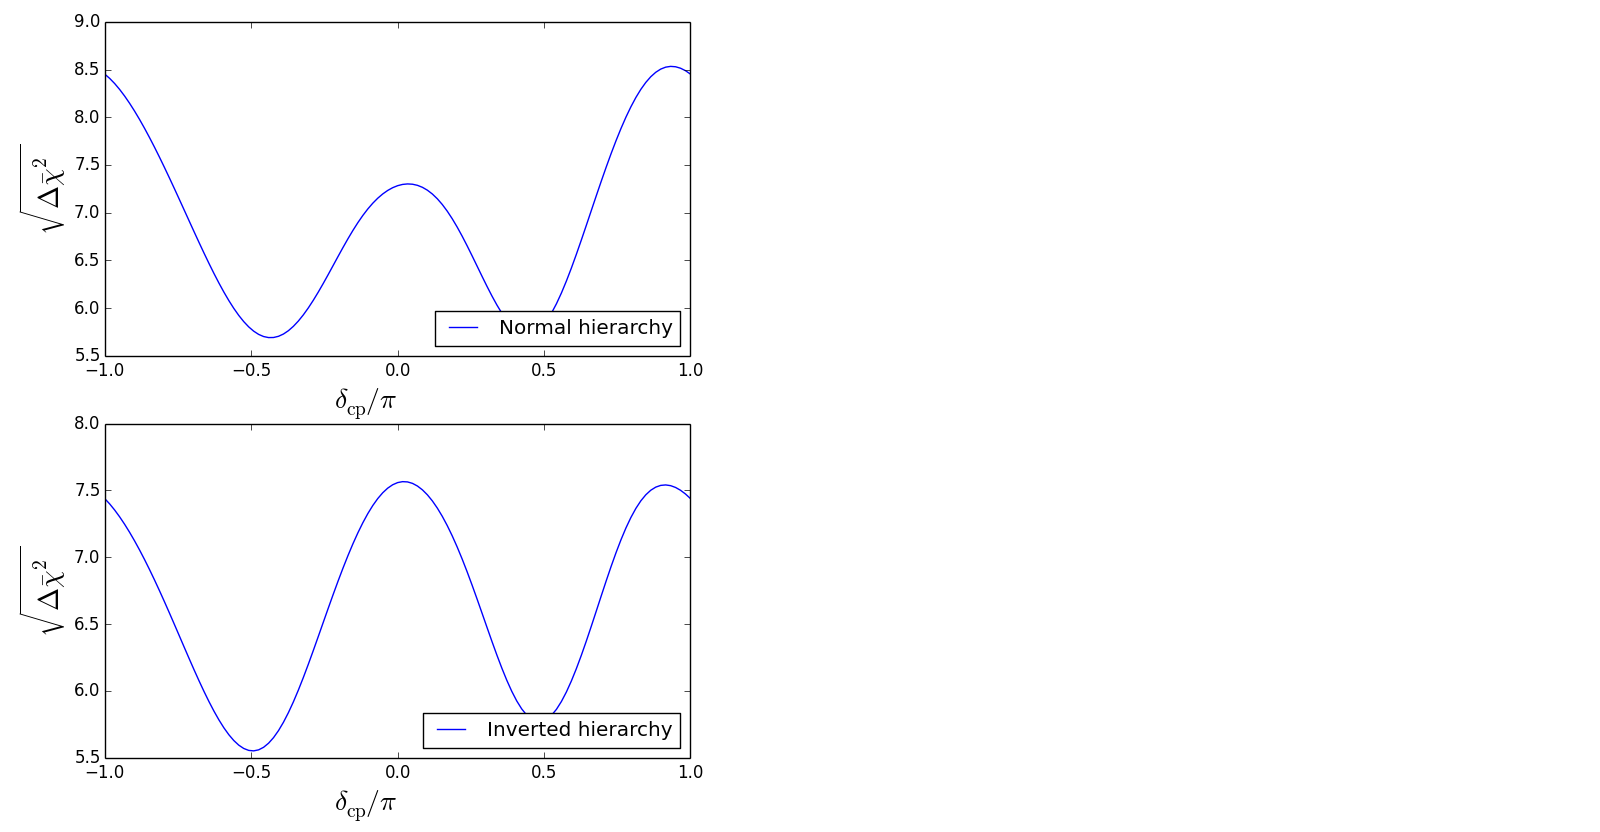
\includegraphics[scale=0.9]{MH_sensitivity2.png}
\begin{figure}[h!]
\caption{Sensitivity to the mass hierarchy as a function of $\delta_{CP}$ for the cases where true mass hierarchy is normal (top) or inverted (bottom). Assumptions are a 1.2 MW, 80 GeV proton beam producing $1.5\times 10^{21}$ POT per year, running for 1 year, with a 10 kt detector mass.}
\label{fig:sensitivity4}
\end{figure}
\end{center}
\begin{center}
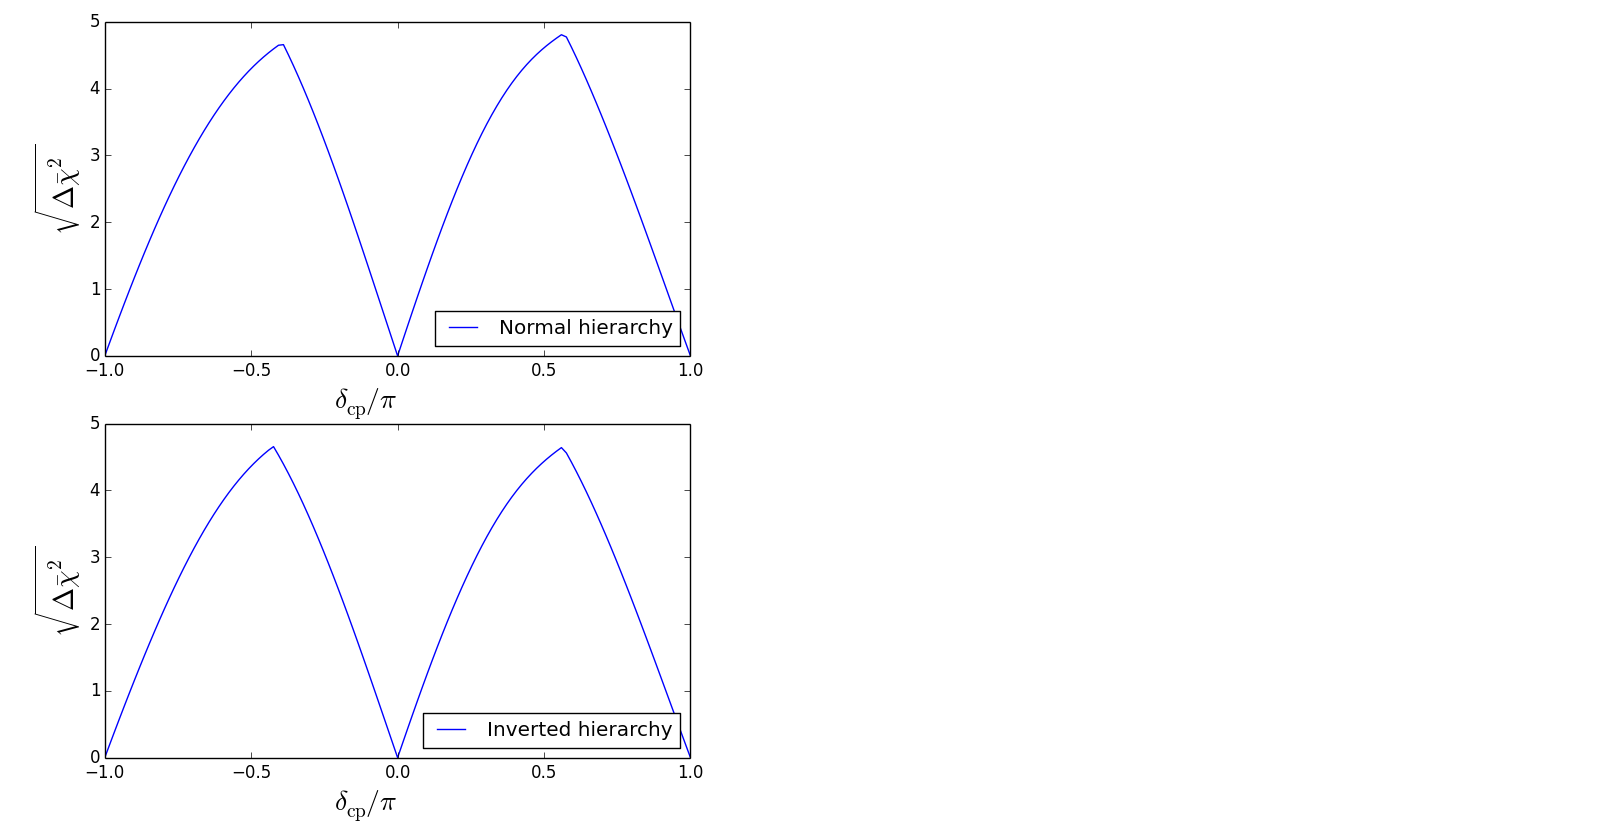
\includegraphics[scale=0.9]{CPV_sensitivity2.png}
\begin{figure}[h!]
\caption{Sensitivity to CP violation as a function of $\delta_{CP}$ for both mass hierarchies. Assumptions are a 1.2 MW, 80 GeV proton beam producing $1.5\times 10^{21}$ POT per year, running for 1 year, with a 10 kt detector mass.}
\label{fig:sensitivity3}
\end{figure}
\end{center}\\\\
\section{Summary and conclusions}
This project has summarised the some history of the neutrino, including its prediction by Pauli and its discovery by Cowen and Reines, as well as the discovery of the different neutrino flavours and the concept of neutrino mixing. An explanation is given for the phenomenology of neutrino oscillation, including a derivation of two flavour probabilities. Detailed demonstrations of three flavour mixing, showing the effect of the various mixing parameters, including the mass hierarchy, CP violating phase and matter effect are included, and an outline of existing neutrino experiments is given.\\\\
A summary of the principles and design of the LBNE is included, with an investigation of the predicted sensitivity of the LBNE to CP violation and the true neutrino mass hierarchy, neglecting statistical and detector effects. It was found that the LBNE
will be able to determine the neutrino mass hierarchy with very high sensitivity, given a 50 kt LArTPC detector mass, although the model used failed to fully account for the matter effect. It was also found that the LBNE will be highly sensitive to CP violation in this scenario. However there are some funding concerns regarding the construction of the LBNE, so predicted sensitivities for a 10 kt LArTPC detector mass are also calculated. The average sensitivity of the 10 kt detector scenario is shown to be roughly half that of the 50 kt scenario.\\\\
To improve models of the LBNE sensitivity, it may be useful to take into account survival probabilities, to increase the available amount of useful data, and model the oscillations of the electron neutrino/antineutrino component of the beam spectrum, to take into account experimental background. These factors were previously included in this project, but it was not possible to isolate a small discrepancy in the code used, which produced anomalous results when modelling an inverted hierarchy. Where possible this original code was used to produce figures, although it was replaced with a simpler approximation for figures where the mass hierarchy effect was concerned. A more accurate modelling of the Earth's density profile is also needed, the most common way to do this is to divide the beam path into many segments with different, constant densities.
\section{Acknowledgements}
I would like to thank my supervisor, Dr Elisabeth Falk, for all of the help which she has provided me, her time and patience are greatly appreciated. I would also like to thank Dr Jeff Hartnell for his excellent teaching, and my housemates for their support.
\newpage
\section{Appendix}
The following code is an example of the code used to generate the figures shown in this project. The code is entirely original:
\lstset{language=Python}  
\begin{lstlisting}
import numpy as np
import scipy as sc
import matplotlib.pyplot as plt
import math as m
def p( E, hierarchy, deltaCP, Type): # arguments: Energy, initial flavour, final flavour, mass hierarchy, CP phase, electron number density, neutrino or antineutrino
	Ne_SI=2*3.337*10**29 #electrons per m^3. 2 x electron density of water
	hc=1.9732697*10**(-7) # for converting metres to eV^-1
	Ne=Ne_SI*(hc**3) # electrons per eV^-3
	m=(1/(hc)) # 1m in eV-1
	baseline=1287000 # set baseline distance in m
	L=baseline*m # baseline in eV^-1
	Gf=(1.166364*10**-5) / 10**18 #eV^-2
	E=(10**9)*E # converting E to eV from GeV. All quantities in this formula are in terms of eV
	delta21=7.54*10**(-5)# eV^2 mass difference squared
	if hierarchy==0:
		    # { m3 < m1 < m2 hierarchy}
		theta23=0.740#rad        # Mixing angles
		theta12=0.588#rad
		theta13=0.156#rad
		delta=-0.00238# eV^2 mass difference squared  
	else:
			# { m1 < m2 < m3 hierarchy}
		theta23=0.740#rad        # Mixing angles
		theta12=0.588#rad
		theta13=0.154#rad
		delta=0.00243# eV^2 mass difference squared
	s23=np.sin(theta23)      # abbreviated trig functions
	c23=np.cos(theta23)
	s13=np.sin(theta13)
	c13=np.cos(theta13)
	s12=np.sin(theta12)
	c12=np.cos(theta12)
	mass=[1,1+delta21,1+delta21/2+delta]
	delta31=mass[2]-mass[0]
	delta32=mass[2]-mass[1]
	if Type==0:
		deltaCP=-deltaCP
		Gf=-(1.166364*10**-5) / 10**18 #eV^-2
	else:
		deltaCP=deltaCP
		Gf=(1.166364*10**-5) / 10**18 #eV^-2
	A=(np.sqrt(2)*Gf*Ne*2*E/delta31)
	D=(delta31*L/(4*E))
	alpha=(delta21/delta31)
	J=  np.sin(2*theta12)*np.sin(2*theta13)*np.sin(2*theta23)*np.cos(theta13)*np.sin(deltaCP)
	P0 = s23**2 * (np.sin(2*theta13))**2 * (np.sin((A-1)*D))**2 / ((A-1))**2
	P3 = alpha**2 * c23**2 * (np.sin(2*theta12))**2 * (np.sin(A*D))**2 / A**2
	Psin =  -alpha  * J * np.sin(D) * np.sin(A*D) * np.sin((1-A)*D) / (A*(1-A))
	Pcos =  alpha  * J * np.cos(D) * np.sin(A*D) * np.sin((1-A)*D) / (A*(1-A) * np.tan(deltaCP))
	return P0 + P3 + Psin + Pcos
energy=np.linspace(0.25,10.25,40)# energy bins
neutrino_muon=np.array([array entries are not included for the sake of brevity])
neutrino_antimuon=np.array([array entries are not included for the sake of brevity])
antineutrino_antimuon=np.array([array entries are not included for the sake of brevity])
antineutrino_muon=np.array([array entries are not included for the sake of brevity])
total_normal=np.sum(neutrino_muon+neutrino_antimuon)
total_anti=np.sum(antineutrino_muon+antineutrino_antimuon)
normal_scale_factor=0.2*12721/total_normal
anti_scale_factor=0.2*4248/total_anti
def signal(beam_type,hierarchy,deltaCP): # generating a far detector signal for a given beam type, MH and deltaCP
	electron_signal_normal=np.zeros(40)
	electron_signal_anti=np.zeros(40)
	muon_signal_normal=np.zeros(40)
	muon_signal_anti=np.zeros(40)
	for i in range(0,40):
		electron_signal_normal[i] = normal_scale_factor*( p(energy[i],hierarchy,deltaCP,1)*neutrino_muon[i]      + p(energy[i],hierarchy,deltaCP,0)*neutrino_antimuon[i])
		electron_signal_anti[i]   = anti_scale_factor*( p(energy[i],hierarchy,deltaCP,1)*antineutrino_muon[i] + p(energy[i],hierarchy,deltaCP,0)*antineutrino_antimuon[i])
	if beam_type==1:
		return electron_signal_normal
	else: 
		return electron_signal_anti
CP_range=2*np.pi
CP_values=CP_range*60/np.pi
deltaCP=np.linspace(-CP_range/2+0.00001,CP_range/2,CP_values)
def X_MH(deltaCP,MH): # Calculates delta Chi squared for mass hierarchies
	X=np.zeros(CP_values)
	Y=np.zeros(CP_values)
	for j in range(0,len(deltaCP)):
		true_normal_a=signal(1,MH,deltaCP[j])# True signals for both beam tunings and event types
		true_anti_a=signal(0,MH,deltaCP[j])
		test_NH_normal_a=signal(1,1,deltaCP[j])# Test signals for normal hierarchy hypothesis
		test_NH_anti_a=signal(0,1,deltaCP[j])
		test_IH_normal_a=signal(1,0,deltaCP[j])# Test signals for inverted hierarchy hypothesis
		test_IH_anti_a=signal(0,0,deltaCP[j])
		for i in range(0,40):
			X[j] +=  2*(true_normal_a[i]*np.log(true_normal_a[i]/test_NH_normal_a[i])+test_NH_normal_a[i]-true_normal_a[i] + true_anti_a[i]*np.log(true_anti_a[i]/test_NH_anti_a[i])+test_NH_anti_a[i]-true_anti_a[i])
			Y[j] +=  2*(true_normal_a[i]*np.log(true_normal_a[i]/test_IH_normal_a[i])+test_IH_normal_a[i]-true_normal_a[i] + true_anti_a[i]*np.log(true_anti_a[i]/test_IH_anti_a[i])+test_IH_anti_a[i]-true_anti_a[i])
	return np.sqrt(abs(Y-X))# The difference between the Chi squares of the two hypotheses
def X_CPV(deltaCP,MH): # Calculates delta Chi squared for CP violaton
	X=np.zeros(CP_values)
	Y=np.zeros(CP_values)
	for j in range(0,len(deltaCP)):
		true_normal_a=signal(1,MH,deltaCP[j])# True signals for both beam tunings and event types
		true_anti_a=signal(0,MH,deltaCP[j])
		test_zero_normal_a=signal(1,MH,0.00001)# Test signals for zero CP phase
		test_zero_anti_a  =signal(0,MH,0.00001)
		test_pi_normal_a=signal(1,MH,np.pi)# Test signals for pi CP phase
		test_pi_anti_a=signal(0,MH,np.pi)
		for i in range(0,40):
			X[j] +=  2*(true_normal_a[i]*np.log(true_normal_a[i]/test_pi_normal_a[i])+test_pi_normal_a[i]-true_normal_a[i] + true_anti_a[i]*np.log(true_anti_a[i]/test_pi_anti_a[i])+test_pi_anti_a[i]-true_anti_a[i])
			Y[j] +=  2*(true_normal_a[i]*np.log(true_normal_a[i]/test_zero_normal_a[i])+test_zero_normal_a[i]-true_normal_a[i] + true_anti_a[i]*np.log(true_anti_a[i]/test_zero_anti_a[i])+test_zero_anti_a[i]-true_anti_a[i])
	return np.sqrt(np.minimum(X,Y))# The element-wise minimum between the two hypotheses
\end{lstlisting}
\newpage
\section{References and bibliography}
\bibliography{bibliography} 
\bibliographystyle{ieeetr}
\end{document}
